\documentclass{beamer}
\mode<presentation>
{
\usetheme{Boadilla}
%\setbeamercovered{transparent}
\usecolortheme{whale}
}
\setbeamertemplate{footline}[frame number]
\AtBeginSection[]{
  \begin{frame}
  \vfill
  \centering
  \begin{beamercolorbox}[sep=8pt,center,shadow=true,rounded=true]{title}
    \usebeamerfont{title}\insertsectionhead\par%
  \end{beamercolorbox}
  \vfill
  \end{frame}
}

\newcommand{\independent}{\perp\!\!\!\!\perp} 
\usepackage{bibentry}
\nobibliography*
\usepackage{pdfpages}
\usepackage{graphicx}
\usepackage{pgf}
\usepackage{hyperref}
\usepackage{amsmath,amsfonts,nicefrac,amssymb}
\usepackage{graphicx}
%\usepackage{enumerate}
\usepackage{multicol}
\usepackage[square,sort,colon]{natbib}
\usepackage{pdfpages}
\usepackage{url}
\usepackage{ifthen}
\usepackage{subcaption}
\usepackage{longtable}
\usepackage{pdfpages}
\usetheme{Boadilla}
\usepackage{tikz}
\usepackage{environ}
\usepackage{lipsum}
\usepackage{booktabs}
\usepackage{xcolor,colortbl}
%\usepackage{enumitem}
\beamertemplatefootpagenumber
\newcommand{\etal}{\textit{et al} }

%\newenvironment{slide}[1]
%{\begin{frame}[environment=slide]
%\frametitle{\insertsection}}
%{\end{frame}}
%\setbeamertemplate{caption}[numbered]
\setcounter{page}{1}

\title[]{A Framework for Adaptively Incorporating External Evidence in Sequentially Monitored Trials} 
\author[]{
Matthew A. Psioda %\textsuperscript{1}
%, \textsuperscript{2}, \textsuperscript{2}, 
%$^*$
%\textsuperscript{1}
}
%{ \normalsize{		
%			Evan Kwiatkowski\textsuperscript{1}, Eugenio Andraca-Carrera\textsuperscript{2}, 
%			Mat Soukup\textsuperscript{2}, Matthew A. Psioda\textsuperscript{1}\\
%
%
%			\textsuperscript{1} Department of Biostatistics, University of \\
%			North Carolina, McGavran-Greenberg Hall, CB\#7420 \\
%
%
%			\textsuperscript{2}{Division of Biometrics VII, Office of Biostatistics, Center for Drug Evaluation and Research, US Food and Drug Administration, Silver Spring, Maryland, USA}}}
\institute{
%\textsuperscript{1}
Department of Biostatistics, University of North Carolina at Chapel Hill%\\
%\textsuperscript{2}Division of Biometrics VII, Office of Biostatistics, Center for Drug Evaluation and Research, US Food and Drug Administration
}
\date{\scriptsize{September 23$\textsuperscript{rd}$, 2021} \\ \vspace{0.5cm} 
 \tiny{Joint work with Evan Kwiatkowski, Eugenio Andraca-Carrera, and Mat Soukup} }

\begin{document}
\beamertemplatefootpagenumber
\maketitle

\begin{frame}{Outline}
 \tableofcontents
\end{frame}

\section{Motivation -- Pediatric Therapeutic Development}

\begin{frame} \frametitle{Background}
	\begin{itemize}
		
		\item The Pediatric Research Equity Act (PREA) and prior legislation has spurred pediatric
		      research to inform new drug labeling by allowing the FDA to request/require trials 
					in pediatric disease populations \citep{Avant2018}.	

		\vspace{0.5cm}				
		\item At this time, both the EMA/FDA require pediatric research plans at certain stages 
		      of the application for authorization of new medicines.	

	 \vspace{0.5cm}	
		\item Significant challenges are faced in pediatric trials necessitating 
					timeline extensions and/or modifications to original designs developed to meet 
					FDA post marking requirements (PMRs).				
			
    \vspace{0.5cm}
		\item Pediatric trials face numerous barriers (e.g., small 
					participant pools, ethical/parental concerns related to participation \citep{Greenberg2018})
					and are often unable to produce substantial evidence of efficacy.
													
	\end{itemize}
\end{frame}
%
%
%
%
\begin{frame} \frametitle{Motivating Example -- Belimumab Development Program I}
\begin{itemize}
			\item Based on data generated by two well-controlled pivotal 
						trials in adult systemic lupus erythematosus (SLE), the BLISS-52 and 
						BLISS-76 trials, the FDA approved belimumab for the treatment of adults 
						with active, seropositive SLE (who are already on standard therapy).			
\end{itemize}

\vspace{-0.3cm}
\begin{figure}[h]
	\centering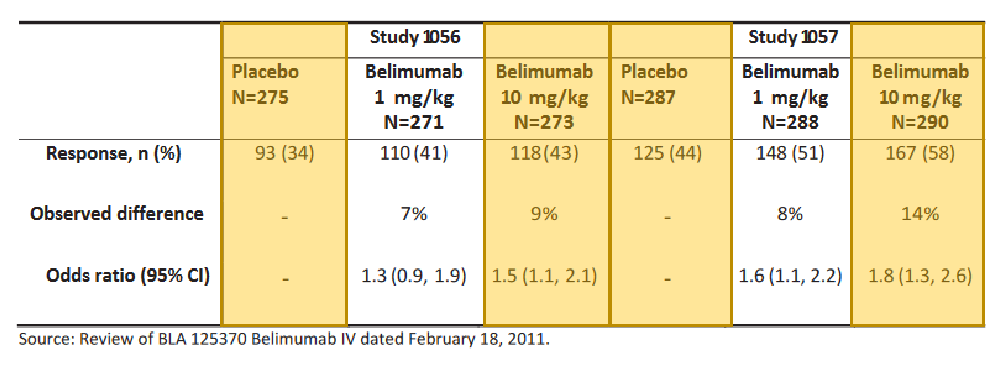
\includegraphics[scale=0.52]{./figures/BLISS.pdf}  
	\vspace{-0.35cm}
	\caption{BLISS Trials Primary Endpoint Data: SRI Response Rate} \label{BLISS_DATA}
\end{figure}	
\end{frame}
%

\begin{frame} \frametitle{Belimumab Development Program II}
\begin{itemize}
			\item As part of the FDA's 2011 approval of belimumab for treatment of 
						adult SLE, a pediatric PMR was issued under PREA.
								
			\vspace{0.2cm}				
			\item This PMR was to conduct a phase II, multicenter study to evaluate the safety, 
						efficacy, and pharmacokinetics of belimumab in a pediatric SLE population.
						
			\vspace{0.2cm}			
			\item The 2011 PMR required a trial with $N=100$ patients but was 
			      reissued in 2016 to require $N=70$ patients due to enrollment challenges.
\end{itemize}

\vspace{-0.3cm}
\begin{figure}[h]
	\centering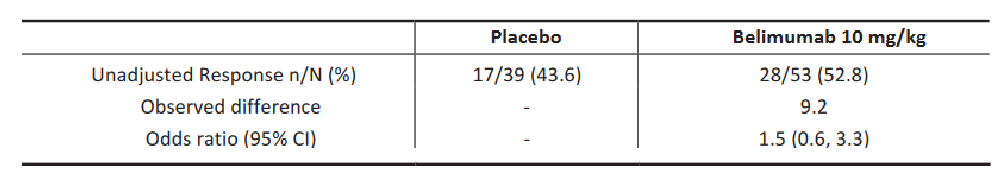
\includegraphics[scale=0.60]{./figures/PLUTO.pdf}  
	\vspace{-0.35cm}
	\caption{PLUTO Trial Primary Endpoint Data: SRI Response Rate} \label{PLUTO_DATA}
\end{figure}
\end{frame}
%
%
%
\begin{frame} \frametitle{Belimumab Development Program III}
\begin{itemize}
			\item For the PLUTO trial, there could be no preconception that the 
						trial was adequate to produce substantial evidence of efficacy 
						on its own. 		
								
			\vspace{0.5cm}
			\item Required sample size for 90\% power $\rightarrow$ $N=760$.
			
			\vspace{0.5cm}			
			\item Nonetheless, the FDA concluded that the safety/efficacy data provided by the PLUTO 
						trial, \textit{taken together with the efficacy/safety data from the BLISS 
						trials}, supported approval of belimumab for pediatric use 
						\citep{FDA127912}.					

			\vspace{0.5cm}			
			\item As a part of the multidisciplinary review, a \textit{post-hoc} Bayesian analysis was requested that
			      borrowed information from the BLISS trials.
						
\end{itemize}
\end{frame}


%%%%%%%%%%%%%%%%%%%%%%%%%%%%%%%%%%%%%%%%%%%%%%%%%%%%%%%%%%%%%%%%%%%%%%%%%%%%%%%%%%%%%%%%%%%
%%%%%%%%%%%%%%%%%%%%%%%%%%%%%%%%%%%%%%%%%%%%%%%%%%%%%%%%%%%%%%%%%%%%%%%%%%%%%%%%%%%%%%%%%%%
%%%%%%%%%%%%%%%%%%%%%%%%%%%%%%%%%%%%%%%%%%%%%%%%%%%%%%%%%%%%%%%%%%%%%%%%%%%%%%%%%%%%%%%%%%%
\section{Bayesian Sequential Monitoring}

%%%%%%%%%%%%%%%%%%%%%%%%%%%%%%%%%%%%%%%%%%%%%%%%%%%%%%%%%%%%%%%%%%%%%%%%%%%%%%%%%%%%%%%%%%%
%%%%%%%%%%%%%%%%%%%%%%%%%%%%%%%%%%%%%%%%%%%%%%%%%%%%%%%%%%%%%%%%%%%%%%%%%%%%%%%%%%%%%%%%%%%
%%%%%%%%%%%%%%%%%%%%%%%%%%%%%%%%%%%%%%%%%%%%%%%%%%%%%%%%%%%%%%%%%%%%%%%%%%%%%%%%%%%%%%%%%%%
\subsection{Philosophy for Sequential Monitoring}
\begin{frame} \frametitle{Philosophy}

\begin{itemize}
	\item Summarizing \cite{Spiegelhalter1994} and others, a Bayesian may monitor data 
				continually and stop collection when any of the following criteria have been met:
		\begin{itemize}
		  \vspace{0.4cm}
			\item A sufficiently skeptical observer becomes convinced $H_1$ is true.
			
			\vspace{0.4cm}
			\item A sufficiently enthusiastic observer becomes convinced $H_1$ is unlikely to be true 
						\textit{or} that the benefit of treatment is not what was hoped.
			
			%\vspace{0.25cm}
			%\item The probability of \textit{eventually} obtaining substantial evidence in favor of $H_1$ drops too low 
			%			from the perspective of a skeptic.
			
			\vspace{0.4cm}
			\item Resources allocated for the study have been exhausted.
		\end{itemize}
		
		\vspace{0.25cm}		
	\item One can analyze accumulating data as frequently as is logistically
	      feasible until one of these criteria is met.
	\end{itemize}
\end{frame}


%%%%%%%%%%%%%%%%%%%%%%%%%%%%%%%%%%%%%%%%%%%%%%%%%%%%%%%%%%%%%%%%%%%%%%%%%%%%%%%%%%%%%%%%%%%
\subsection{Evidence from the Bayesian Perspective}
\begin{frame} \frametitle{Evidence from the Bayesian Perspective I}
	\begin{itemize}
		\item Consider testing the hypotheses 
					\vspace{-0.2cm}
					\[ H_0: \theta \le \theta_0 \text{ versus } H_1: \theta > \theta_0 \]
					
					\vspace{-0.3cm}
					where 
					\begin{itemize}
					  \vspace{0.15cm}
						\item $\theta$ is a parameter of interest (e.g., difference in response rates), and
						
						\vspace{0.25cm}
						\item $\theta_0$ is a chosen constant (e.g., most commonly $\theta_0=0$).
					\end{itemize}
					
		\vspace{0.25cm}			
		\item Suppose there exists a constant $\theta_1 > \theta_0$ that is thought 
					to be a clinically meaningful and also a plausible.
					\begin{itemize}				
						\vspace{0.25cm}
						\item $\theta_1 = 0.118$ based on the BLISS trial data
					\end{itemize}							
					
					
					
		
  \end{itemize}
\end{frame}
%
%
%
\begin{frame} \frametitle{Evidence from the Bayesian Perspective II}
	\begin{itemize}
			
	  \item A standard Bayesian decision rule is given by
					\[ P_\pi\left( \theta > \theta_0 \big| \mathbf{D} \right) > 1 - \epsilon, \]
					based on some prior distribution $\pi\left( \theta \right)$ and data $\mathbf{D}$.
					
		\vspace{0.3cm}			
		\item One may formally define the concept of \textcolor{purple}{substantial total evidence} 
		      in favor of a claim (e.g., $\theta > \theta_0$) as the posterior probability of the claim 
					exceeding $1 - \epsilon$.	
							
	  \vspace{0.3cm}
		\item \textcolor{purple}{Total information} =  \textcolor{blue}{information from likelihood} + 
		\textcolor{red}{prior information}						
							
			\vspace{0.30cm}
			\item Sequential monitoring rationale:
				\begin{itemize}
				 \vspace{0.30cm}
				 \item Skeptic: substantial total evidence that $\theta> \theta_0 \implies$ enrollment stop.
				
				 \vspace{0.30cm}
				 \item Enthusiast: substantial total evidence that $\theta < \theta_1 \implies$ study stop.	
				\end{itemize}
				
					

  \end{itemize}
\end{frame}

\subsection{Skeptical/Enthusiastic Priors}
\begin{frame} \frametitle{Skeptical and Enthusiastic Priors I}
	\begin{itemize}
		\item Define a skeptical observer as someone whose belief satisfies:
					\begin{enumerate}
					  \vspace{0.35cm}
						\item[(i)] 		The observer believes $\theta_0$ is the most likely value 
													of $\theta$.
													
						\vspace{0.35cm}							
						\item[(ii)] 	Belief consistent with substantial total evidence that $\theta < \theta_1$.		
						
						\vspace{0.35cm}	
						\item[(iii)] Formally, this is defined as the prior $\pi_{S}(\theta)$ satisfying 
						             $\text{argmax}_\theta~\pi_S(\theta)=\theta_0$  and $P_S(\theta <\theta_1)=1-\epsilon$.					
					\end{enumerate}
					
		\vspace{0.35cm}			
		\item Define an enthusiastic observer as someone whose belief satisfies:
					\begin{enumerate}
					  \vspace{0.35cm}
						\item[(i)] 		The observer believes $\theta_1$ is the most likely value 
													of $\theta$.
													
						\vspace{0.35cm}							
						\item[(ii)] 	Belief consistent with substantial total evidence that $\theta > \theta_0$.		
						
						\vspace{0.35cm}	
					  \item[(iii)] Formally, this is defined as the prior $\pi_{E}(\theta)$ satisfying 
						             $\text{argmax}_\theta~\pi_E(\theta)=\theta_1$ and $P_E(\theta >\theta_0)=1-\epsilon$.							
					\end{enumerate}						
	\end{itemize}
\end{frame}


\begin{frame}{Skeptical and Enthusiastic Priors II}
\begin{itemize}
\item For prior construction, we propose the flexible family of generalized normal distributions -- $\mathcal{GN}(\mu,\alpha,\beta)$
\begin{align*}
f(\theta)=\frac{\beta}{2\alpha\Gamma(1/\beta)}\exp\left\{-\left(\frac{|\theta-\mu|}{\alpha}\right)^\beta\right\}
\end{align*} where 
		\begin{itemize}
					  \vspace{0.2cm}
						\item $\mu$ is a location parameter, 
						
						\vspace{0.2cm}
						\item $\alpha$ is a scale parameter, and 
													
						\vspace{0.2cm}							
						\item $\beta>0$ is a shape parameter.		
		\end{itemize} 
	
	\vspace{0.3cm}	
	\item This family of distributions accommodates a variety of shapes -- both very peaked and very flat -- and includes the normal distribution as a special case.
%\item
%A monitoring prior in the generalized normal family of distributions can have density at the mode equal to $k\times \frac{1}{\sqrt{2\pi}\sigma}$, with $k<1$ indicating a more flattened distribution and $k>1$ indicating a more peaked distribution at the mode, relative to the default normal distribution. 
\end{itemize}
\end{frame}


\begin{frame}{Skeptical and Enthusiastic Priors III}
\begin{figure}[htbp]
\begin{center}
%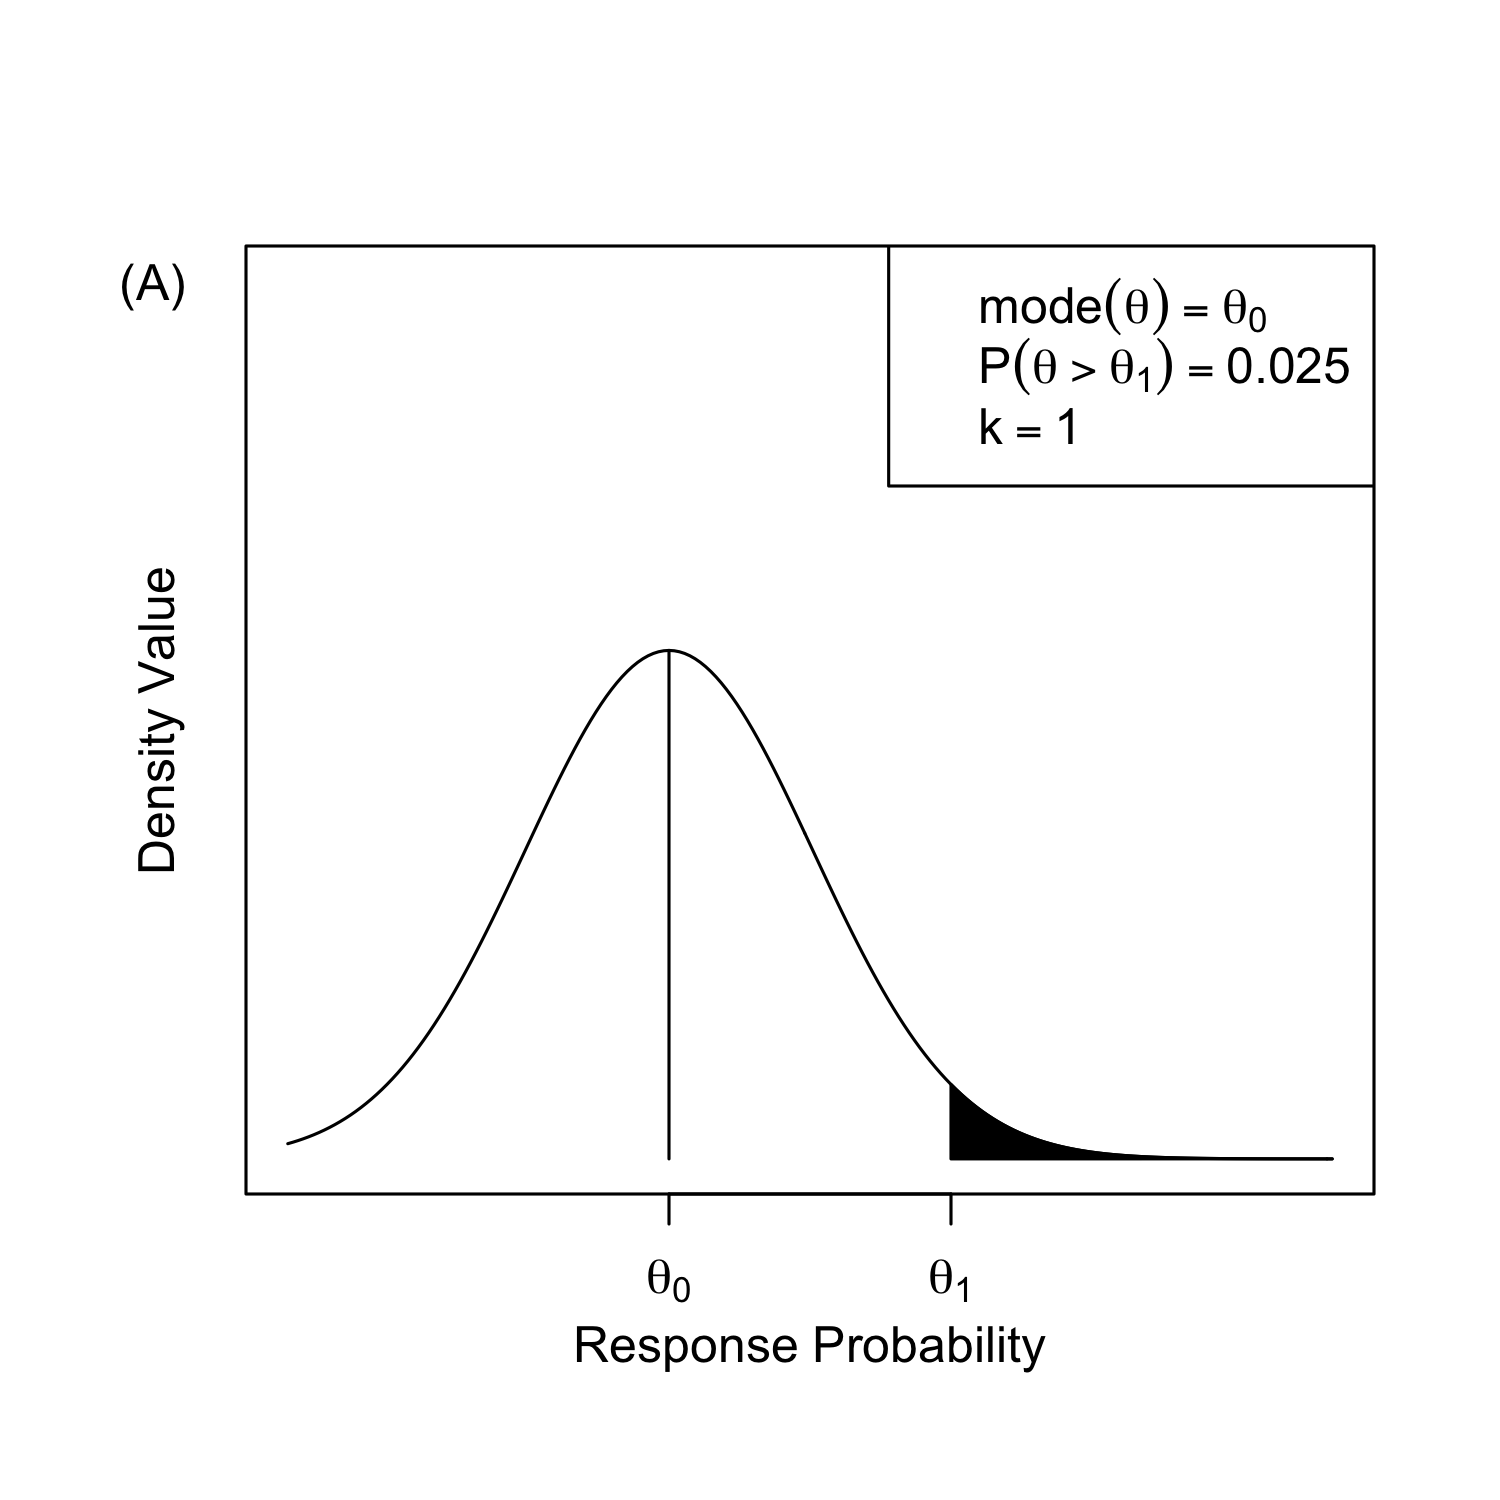
\includegraphics[width=2in]{./figures/figure1a.png}
%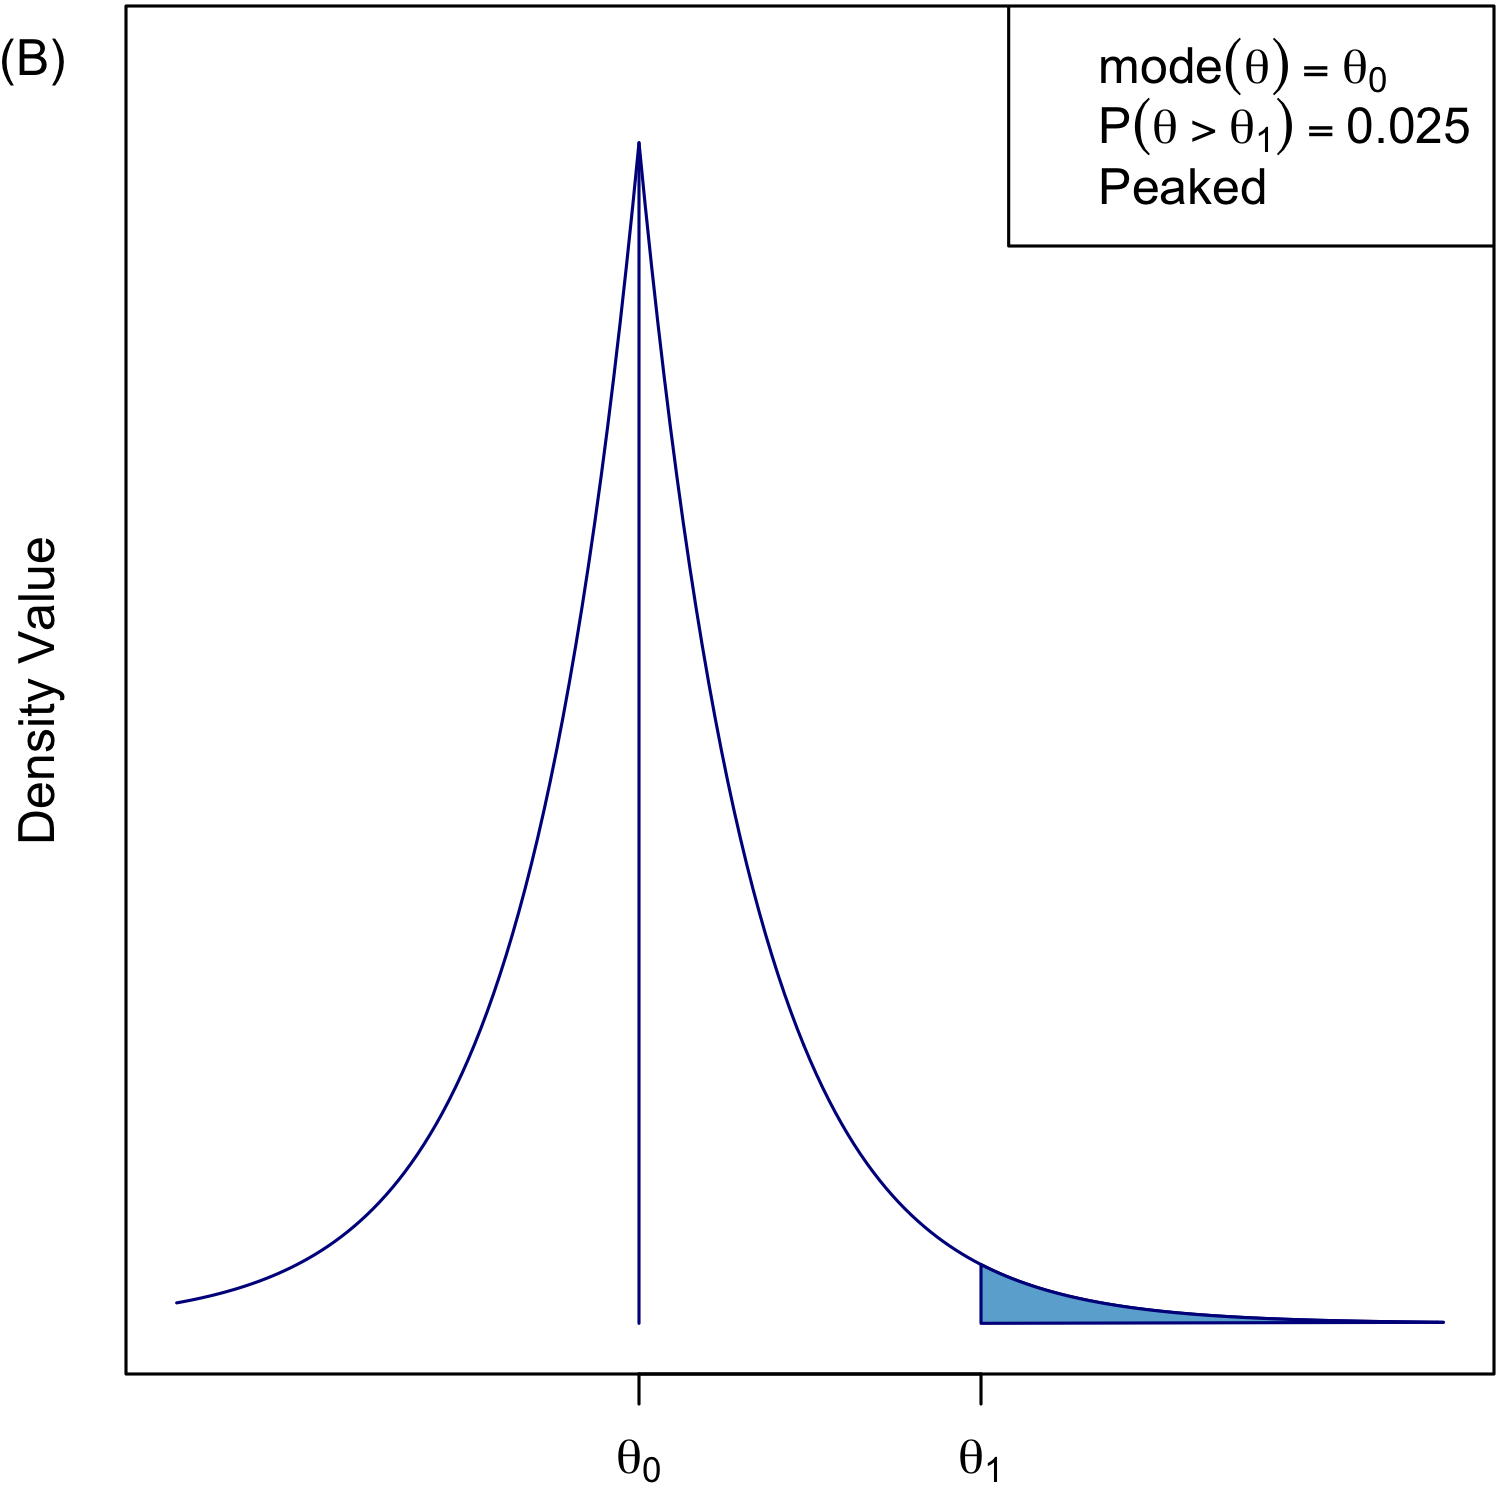
\includegraphics[width=2in]{./figures/figure1b.png}
\vspace{-0.3cm}

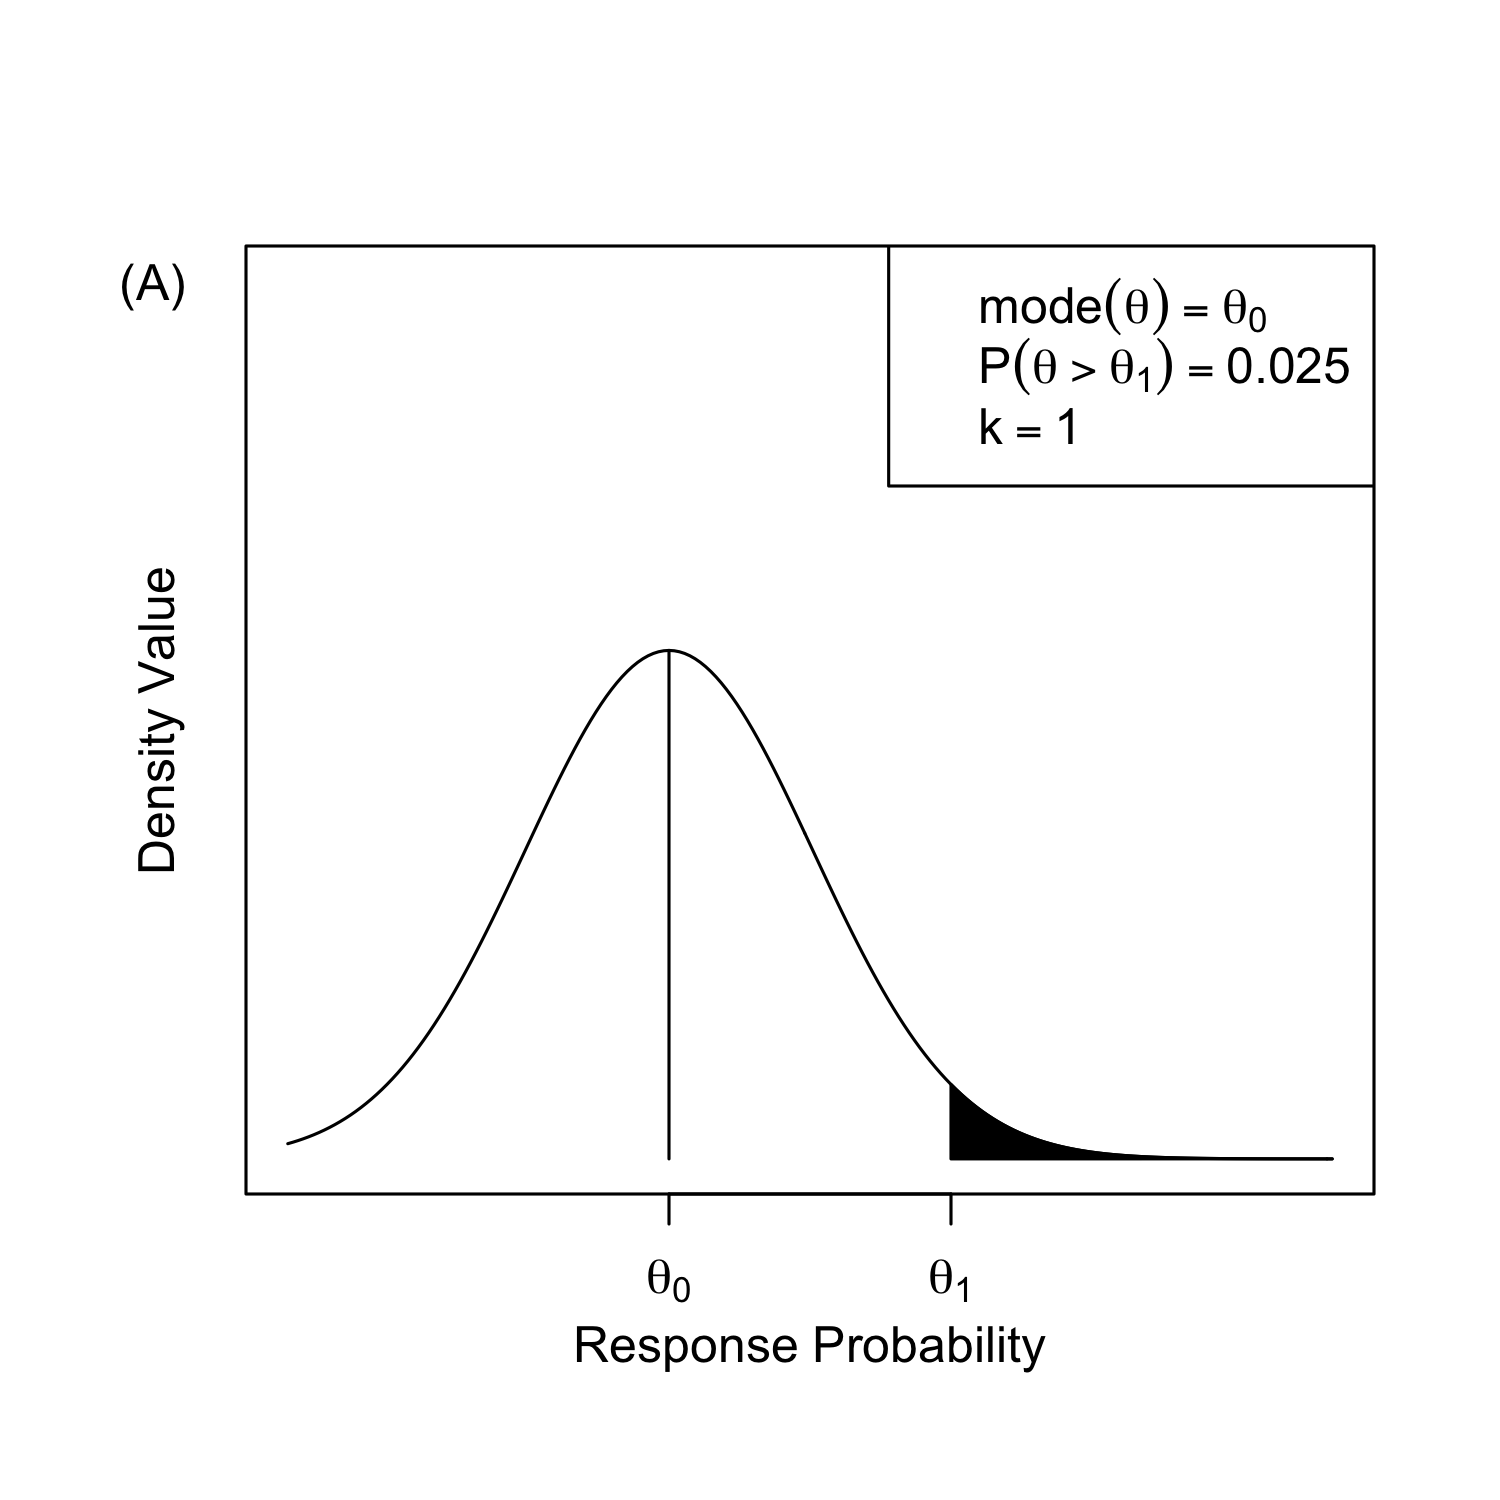
\includegraphics[width=0.28\textwidth]{./figures/figure1a.png}
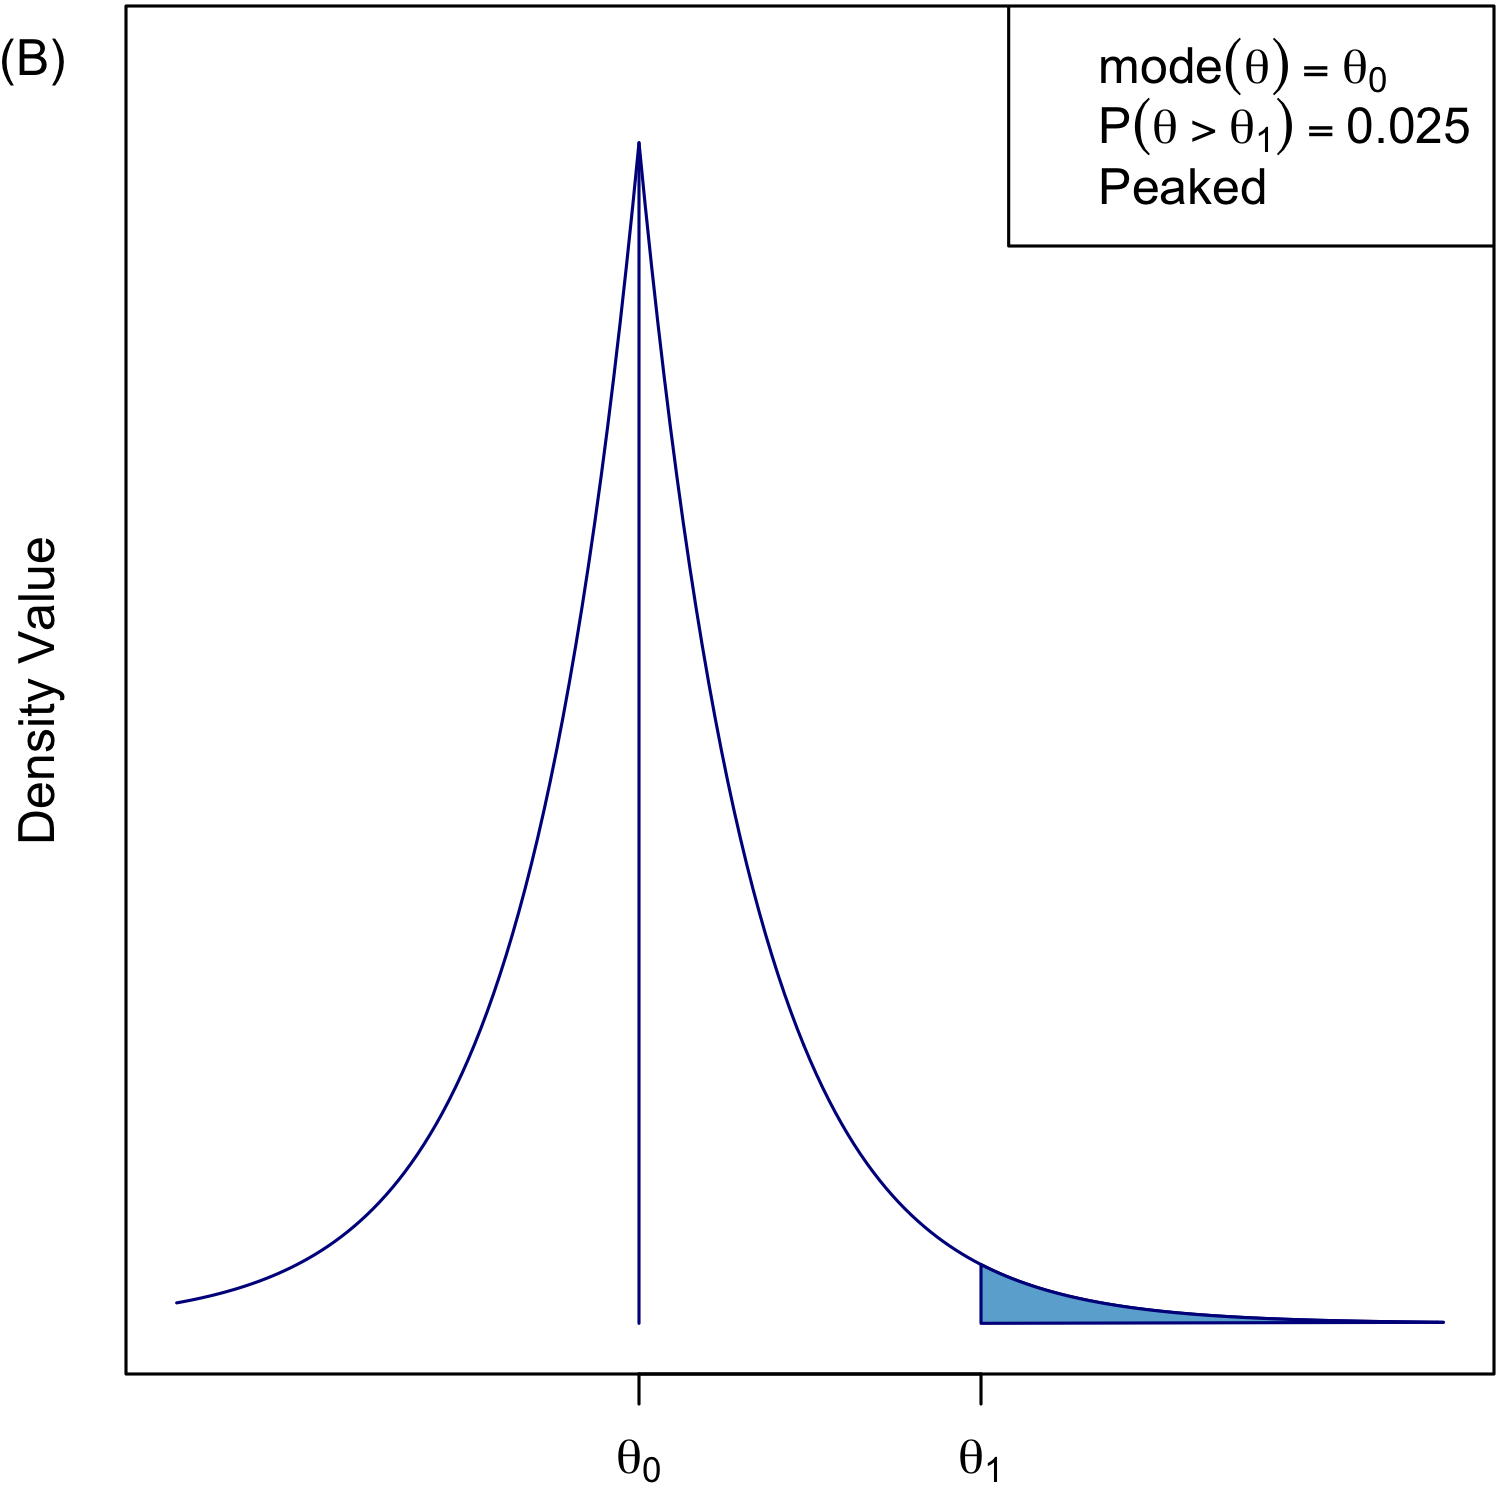
\includegraphics[width=0.28\textwidth]{./figures/figure1b.png}

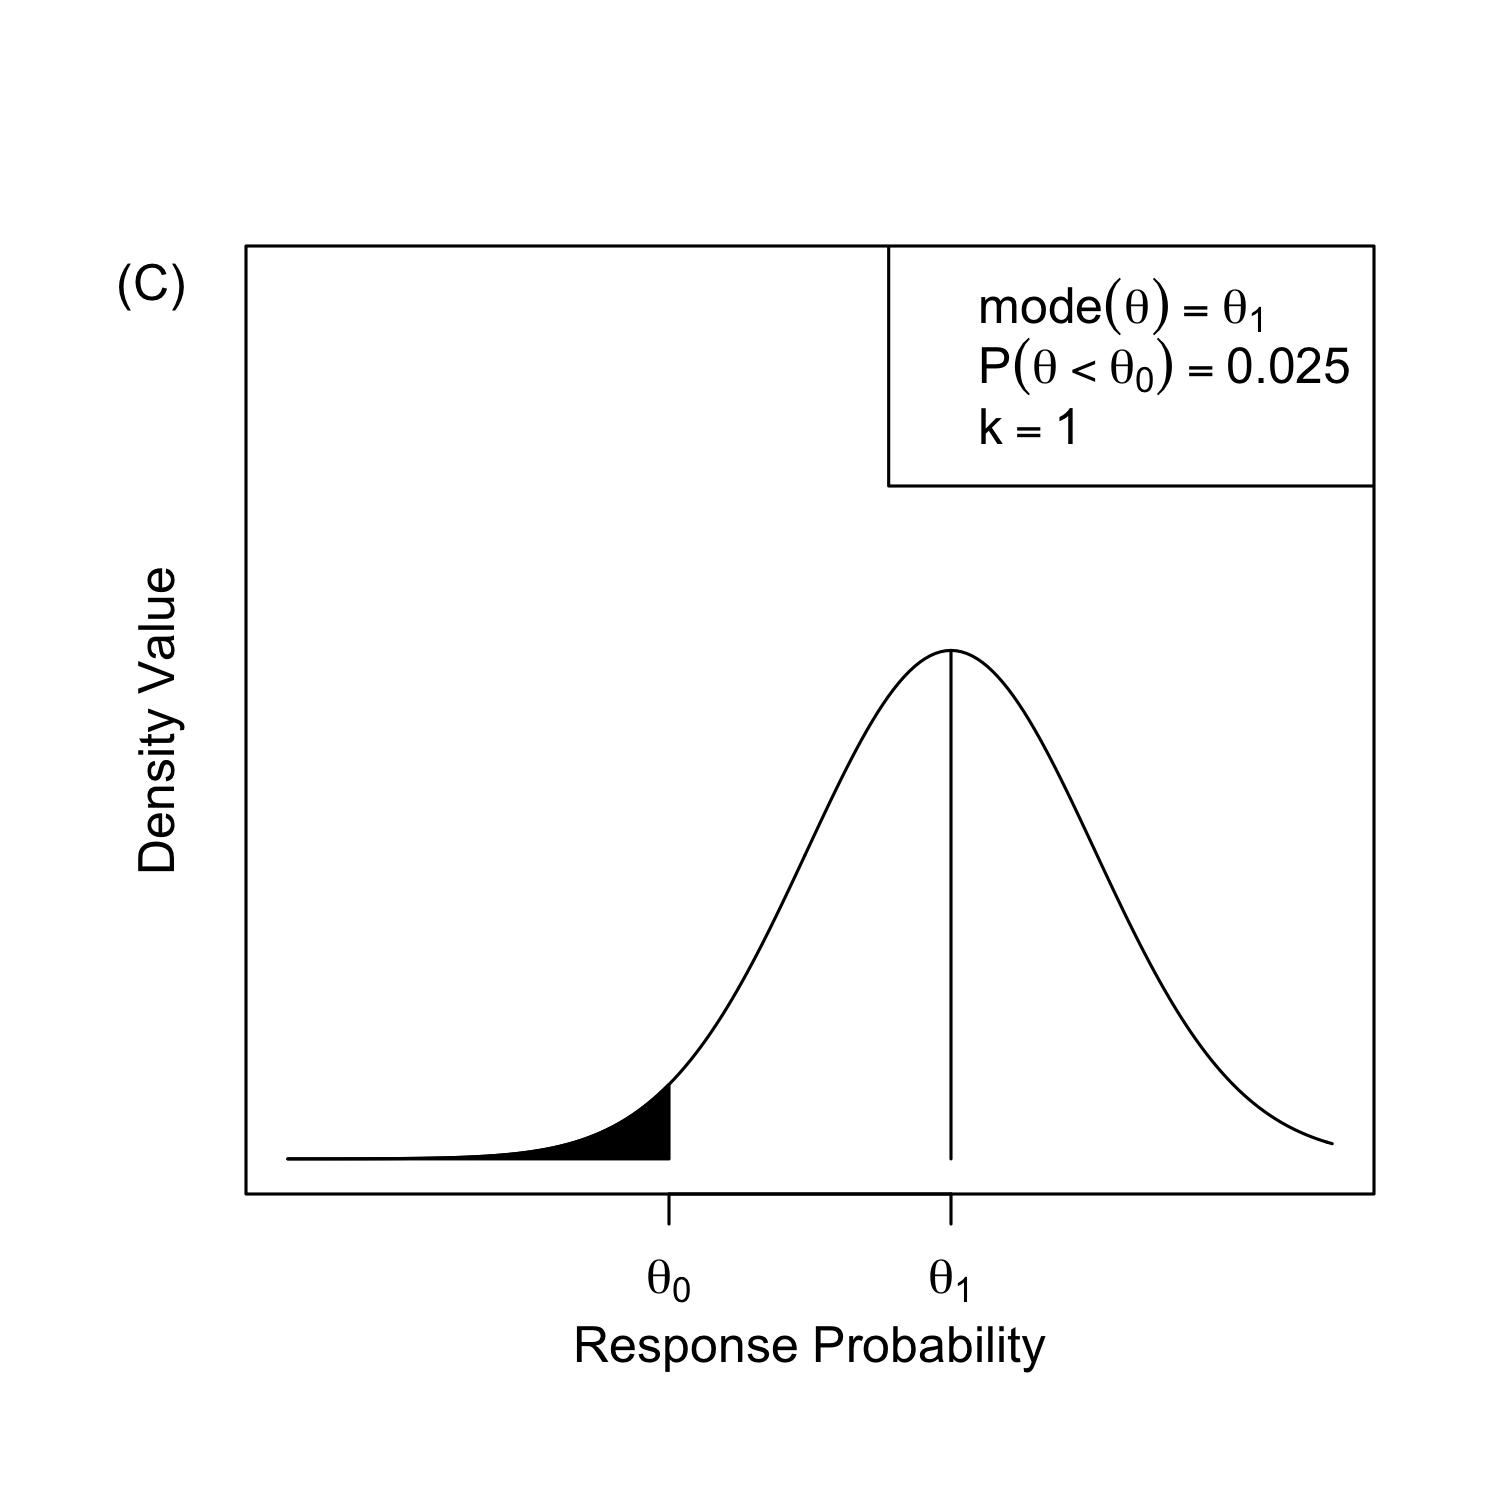
\includegraphics[width=0.28\textwidth]{./figures/figure1c.png}
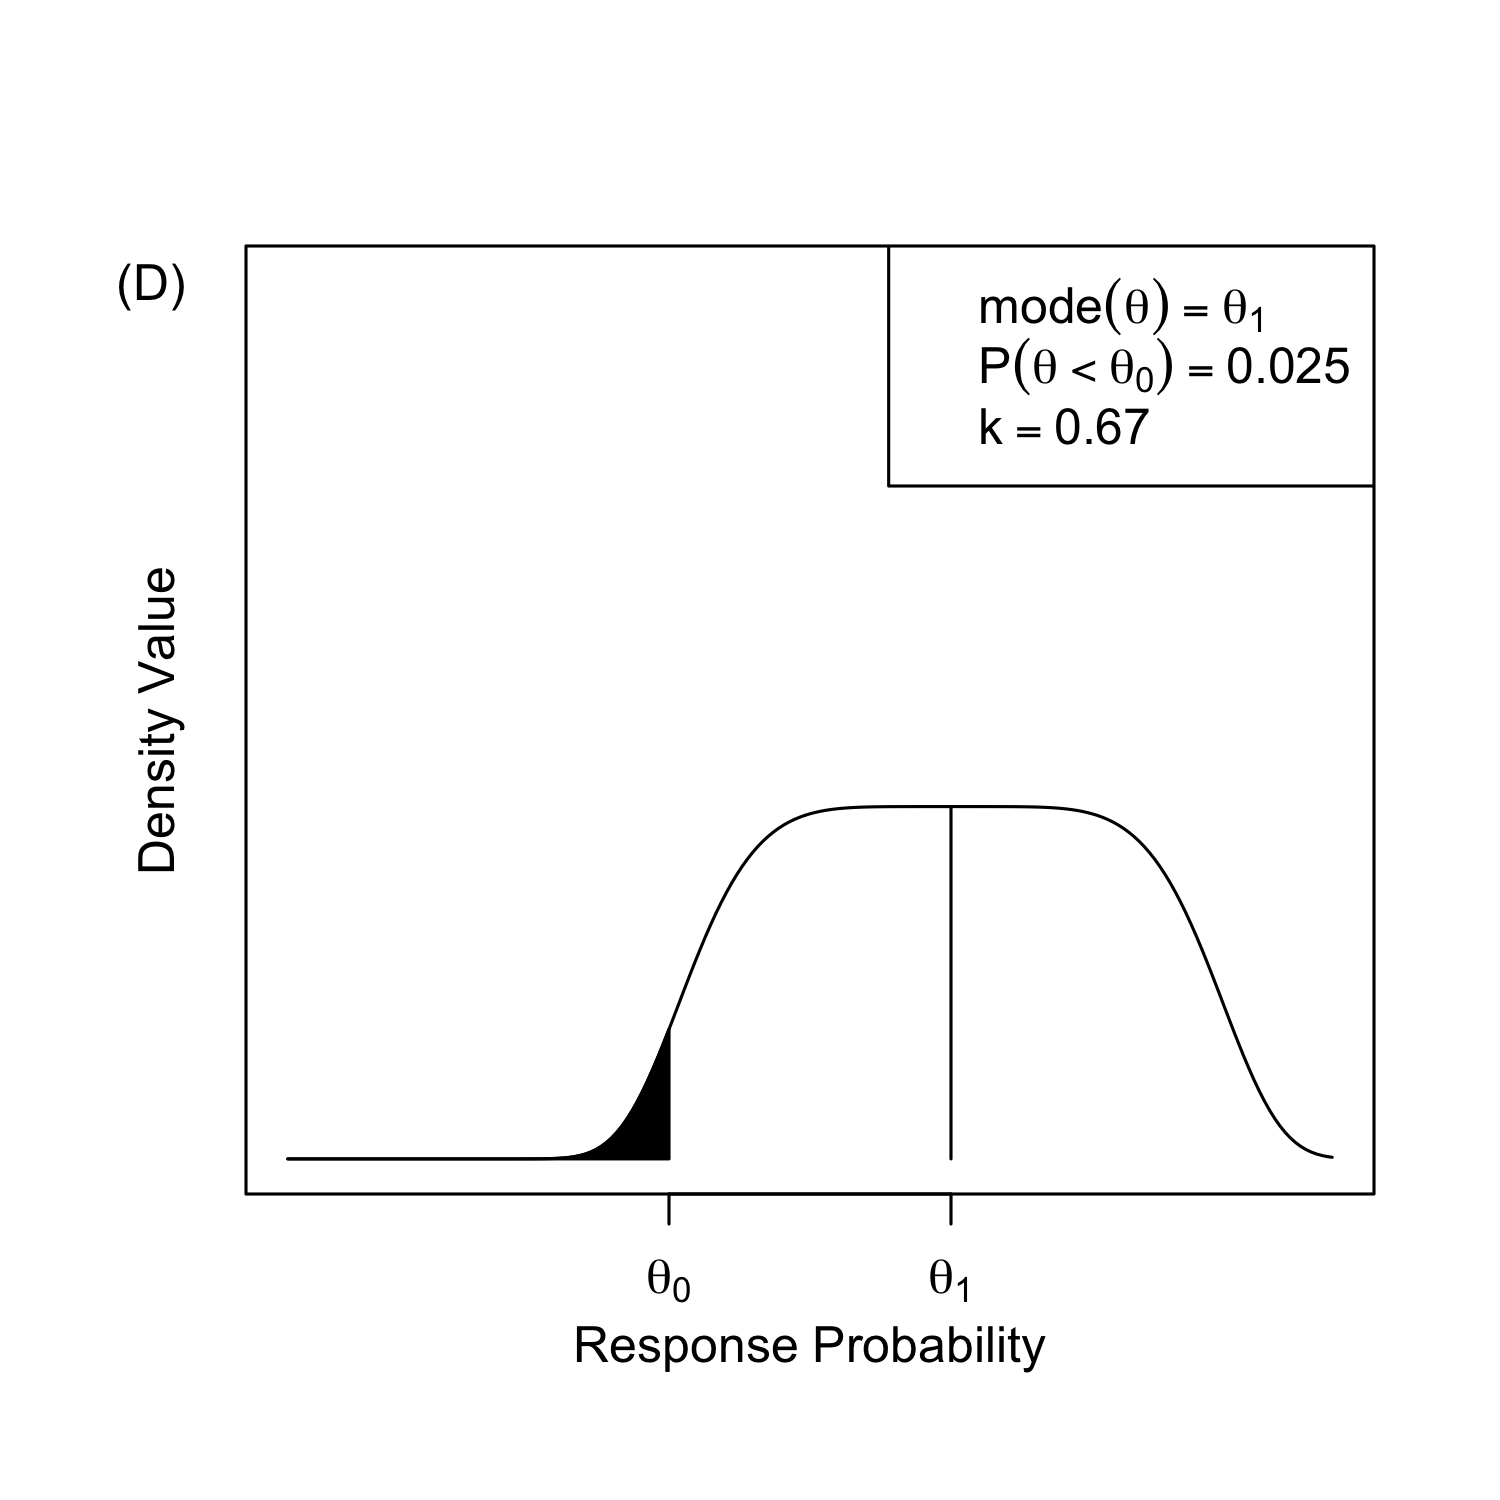
\includegraphics[width=0.28\textwidth]{./figures/figure1d.png}
\caption{A, Default skeptical prior.    B, Concentrated skeptical prior.
         C, Default enthusiastic prior. D, Flattened enthusiastic prior.}

\label{fig:figure1}
\end{center}
\end{figure}
	
\end{frame}




\subsection{Adaptive Monitoring Priors}

\begin{frame}{Adaptive Monitoring Prior I}
\begin{itemize}
	\item 
	One may define an \textit{adaptive monitoring prior} for efficacy monitoring as the mixture distribution	
	\begin{equation*}
		\pi_{AMP}\left(\theta\right)=\omega\cdot\pi_E(\theta)+(1 - \omega)\cdot \pi_S(\theta)
	\end{equation*}
	
	\vspace{0.2cm}
	\item We take $\omega = (1 - \delta) \times \psi^{(E)}(\mathbf{D}_{\text{obs}})$, where 
	
	\begin{itemize}
	  \vspace{0.2cm}	
		\item $\psi^{(E)}(\mathbf{D}_{\text{obs}}) \in [0,1]$ is a measure
		      of congruency between the pediatric data and the enthusiastic prior, and
					
		\vspace{0.2cm}		
		\item $\delta \in [0,1]$ provides a limit regarding how much the adaptive monitoring prior can ``shift'' away from
					the skeptical perspective and towards the enthusiastic one.			
	\end{itemize}
	
		\vspace{0.2cm}								
		\item $\delta=1 \rightarrow \pi_{AMP}\left(\theta\right) = \pi_{S}\left(\theta\right)$ regardless of $\psi^{(E)}(\mathbf{D}_{\text{obs}})$	
					
\end{itemize}
\end{frame}

\begin{frame} \frametitle{Adaptive Monitoring Prior II}
	\begin{itemize}
		\item Similar to \cite{Psioda2020JBS}, we weight the enthusiastic prior based on  
					congruency of the pediatric data with the enthusiastic prior predictive distribution
					using a Bayesian p-value (\cite{Box1980}).
		
		\vspace{0.2cm}								
		\item The prior-predictive distribution for reflects the probability of 
					observing data $\mathbf{D}$ given the enthusiastic prior.
						\begin{equation*}
								p(\mathbf{D}) =\int p(\mathbf{D}|\theta)\pi_E(\theta)d\theta
						\end{equation*}

		\vspace{0.0cm}								
		\item Let $\mathbf{D}_{\text{obs}}$ be the observed data at some point in time in an ongoing trial. 
		         Box's p-value is defined as the following:
						\begin{equation*}
								\psi({\mathbf{D}_{\text{obs}}})=\int {p(\mathbf{D})}  1[p(\mathbf{D})\leq p(\mathbf{D}_{\text{obs}})] d\mathbf{D},
						\end{equation*}
						
						\vspace{-0.25cm}
						where $1[A]$ is an indicator that the event $A$ is true.
\end{itemize}
\end{frame}




\section{An Illustration Based on the PLUTO Trial}
\begin{frame}{Returning to the PLUTO Trial}
\begin{itemize}
	  \item From the BLISS trial data, we elicited an enthusiastic prior that reflected a 
	    	  difference in response probabilities equal to $\theta_1=0.118$.
		
		\vspace{0.2cm}	
		\item A weakly informative prior was elicited for the placebo group response probability (denoted by $\eta$) centered
		      at approximately $\eta_0=0.38$. 
\end{itemize}

\vspace{-0.3cm}
\begin{figure}[htbp]
\begin{center}
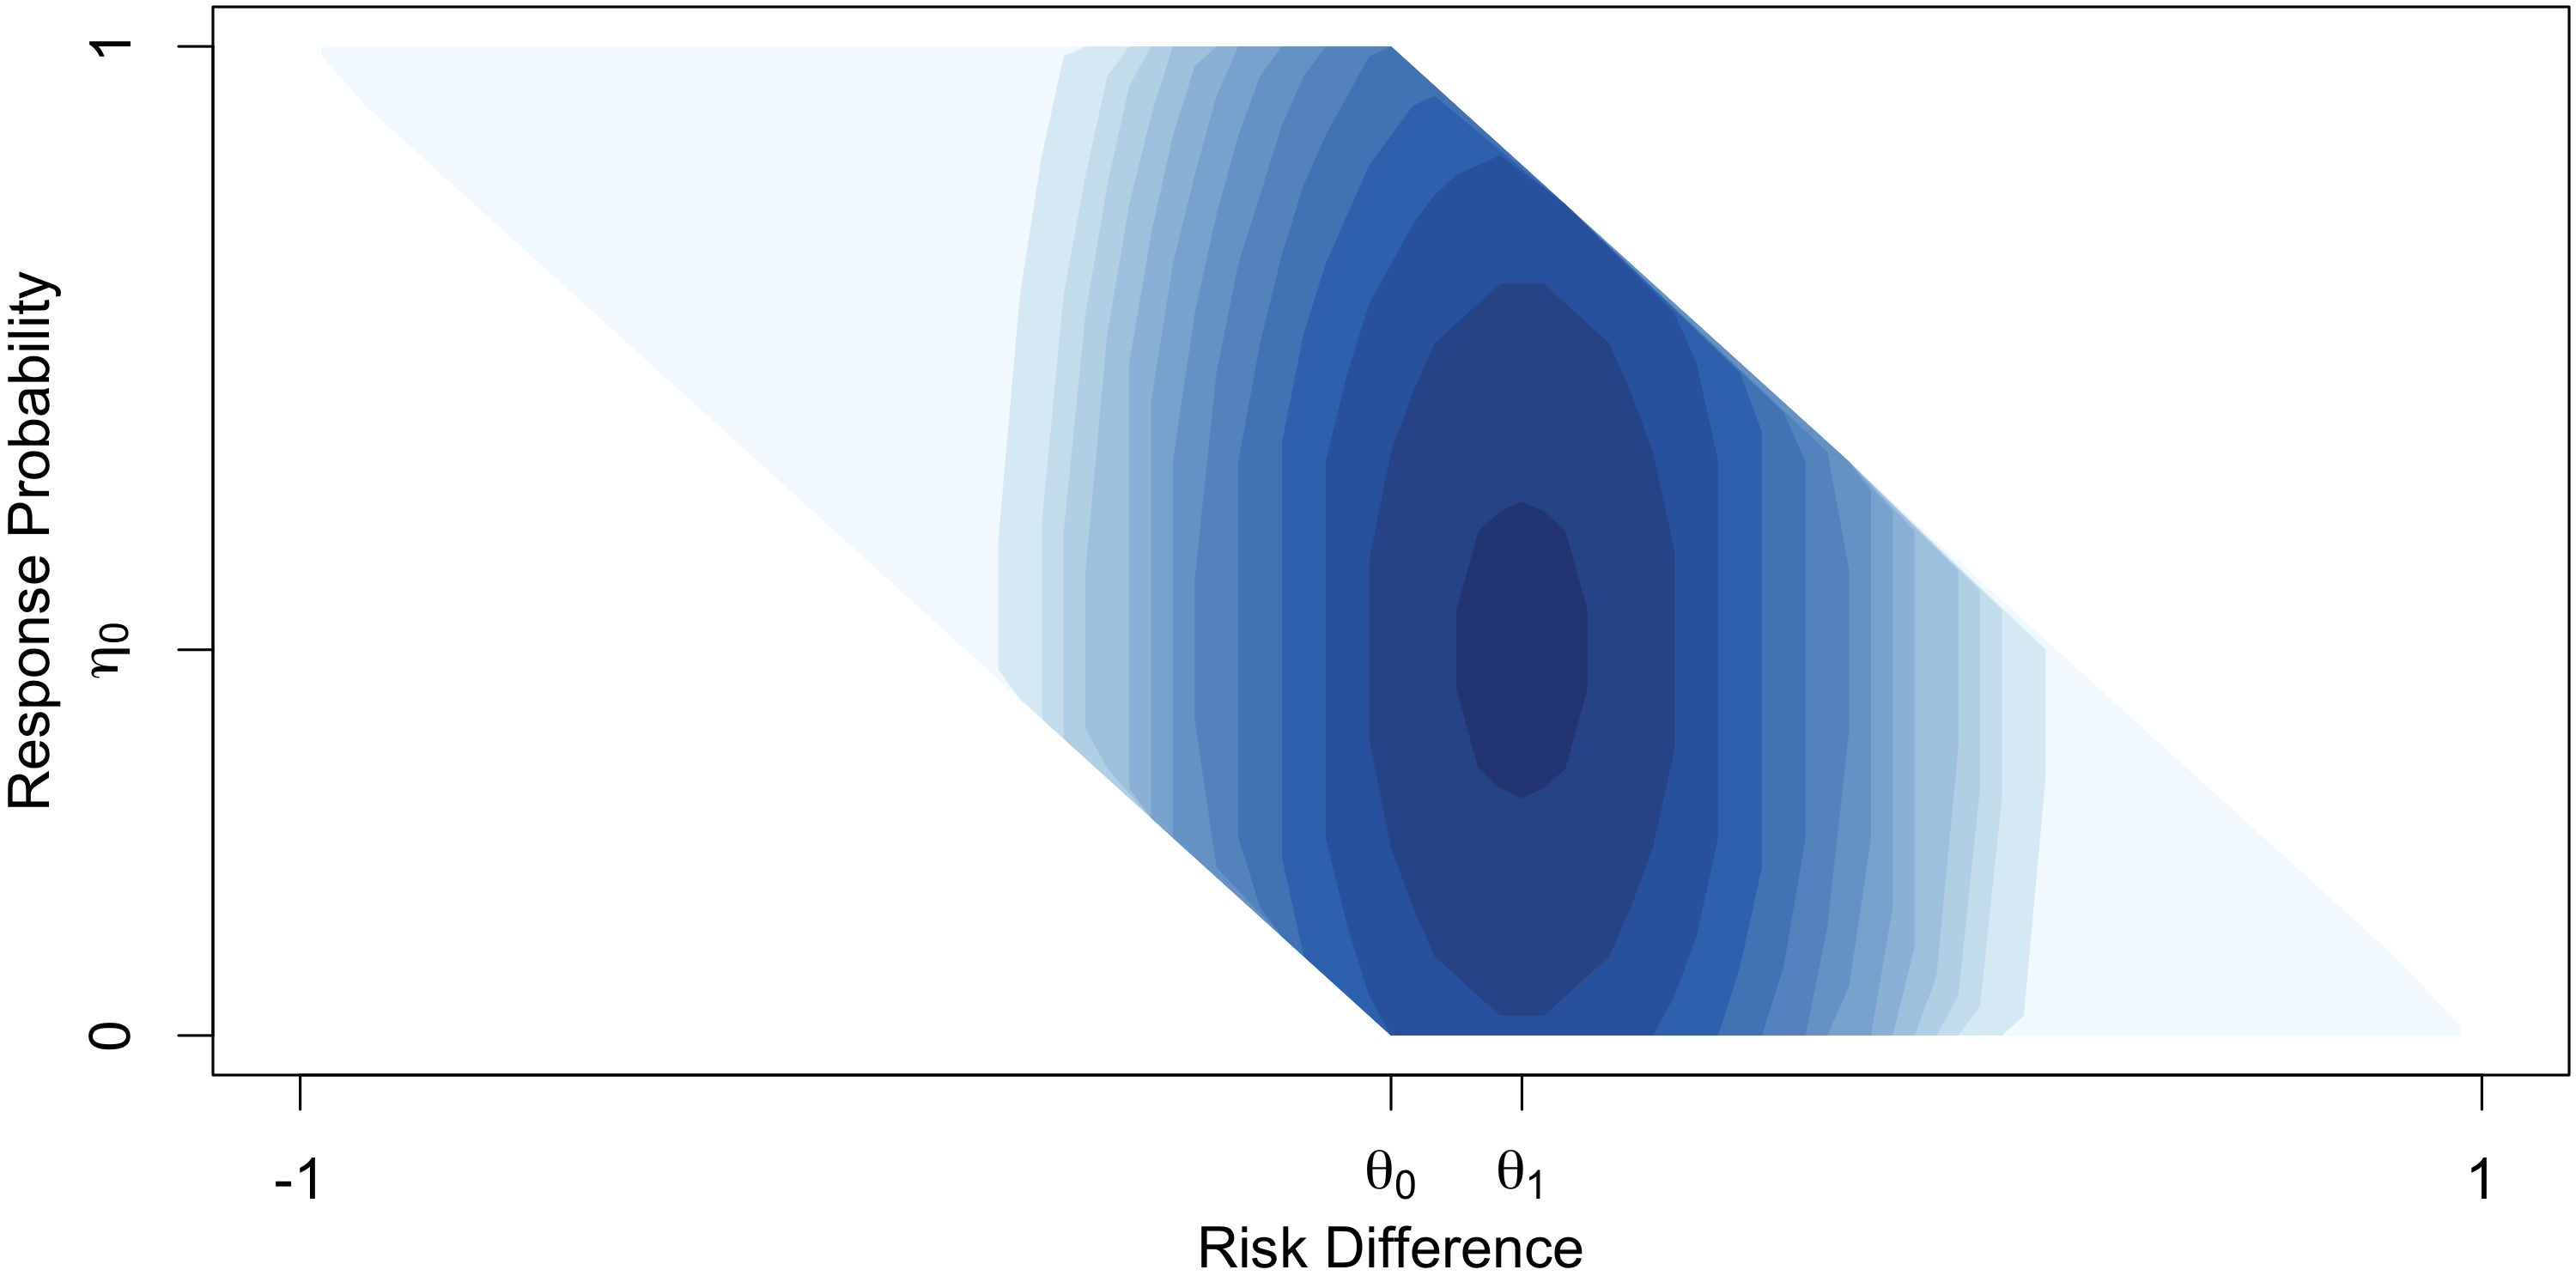
\includegraphics[width=0.8\textwidth]{./figures/enth_aug12.png}
\caption{$\pi(\theta,\eta)=\pi(\theta)\times\pi(\eta|\theta)$ over $-1<\theta<1$ and $0<\theta+\eta<1$.}
\label{fig:figure5}
 \end{center}
\end{figure}

\end{frame}




\begin{frame}{Enthusiastic Prior Mixing Weight $\omega$}

\vspace{-0.5cm}
\begin{figure}[htbp]
\begin{center}
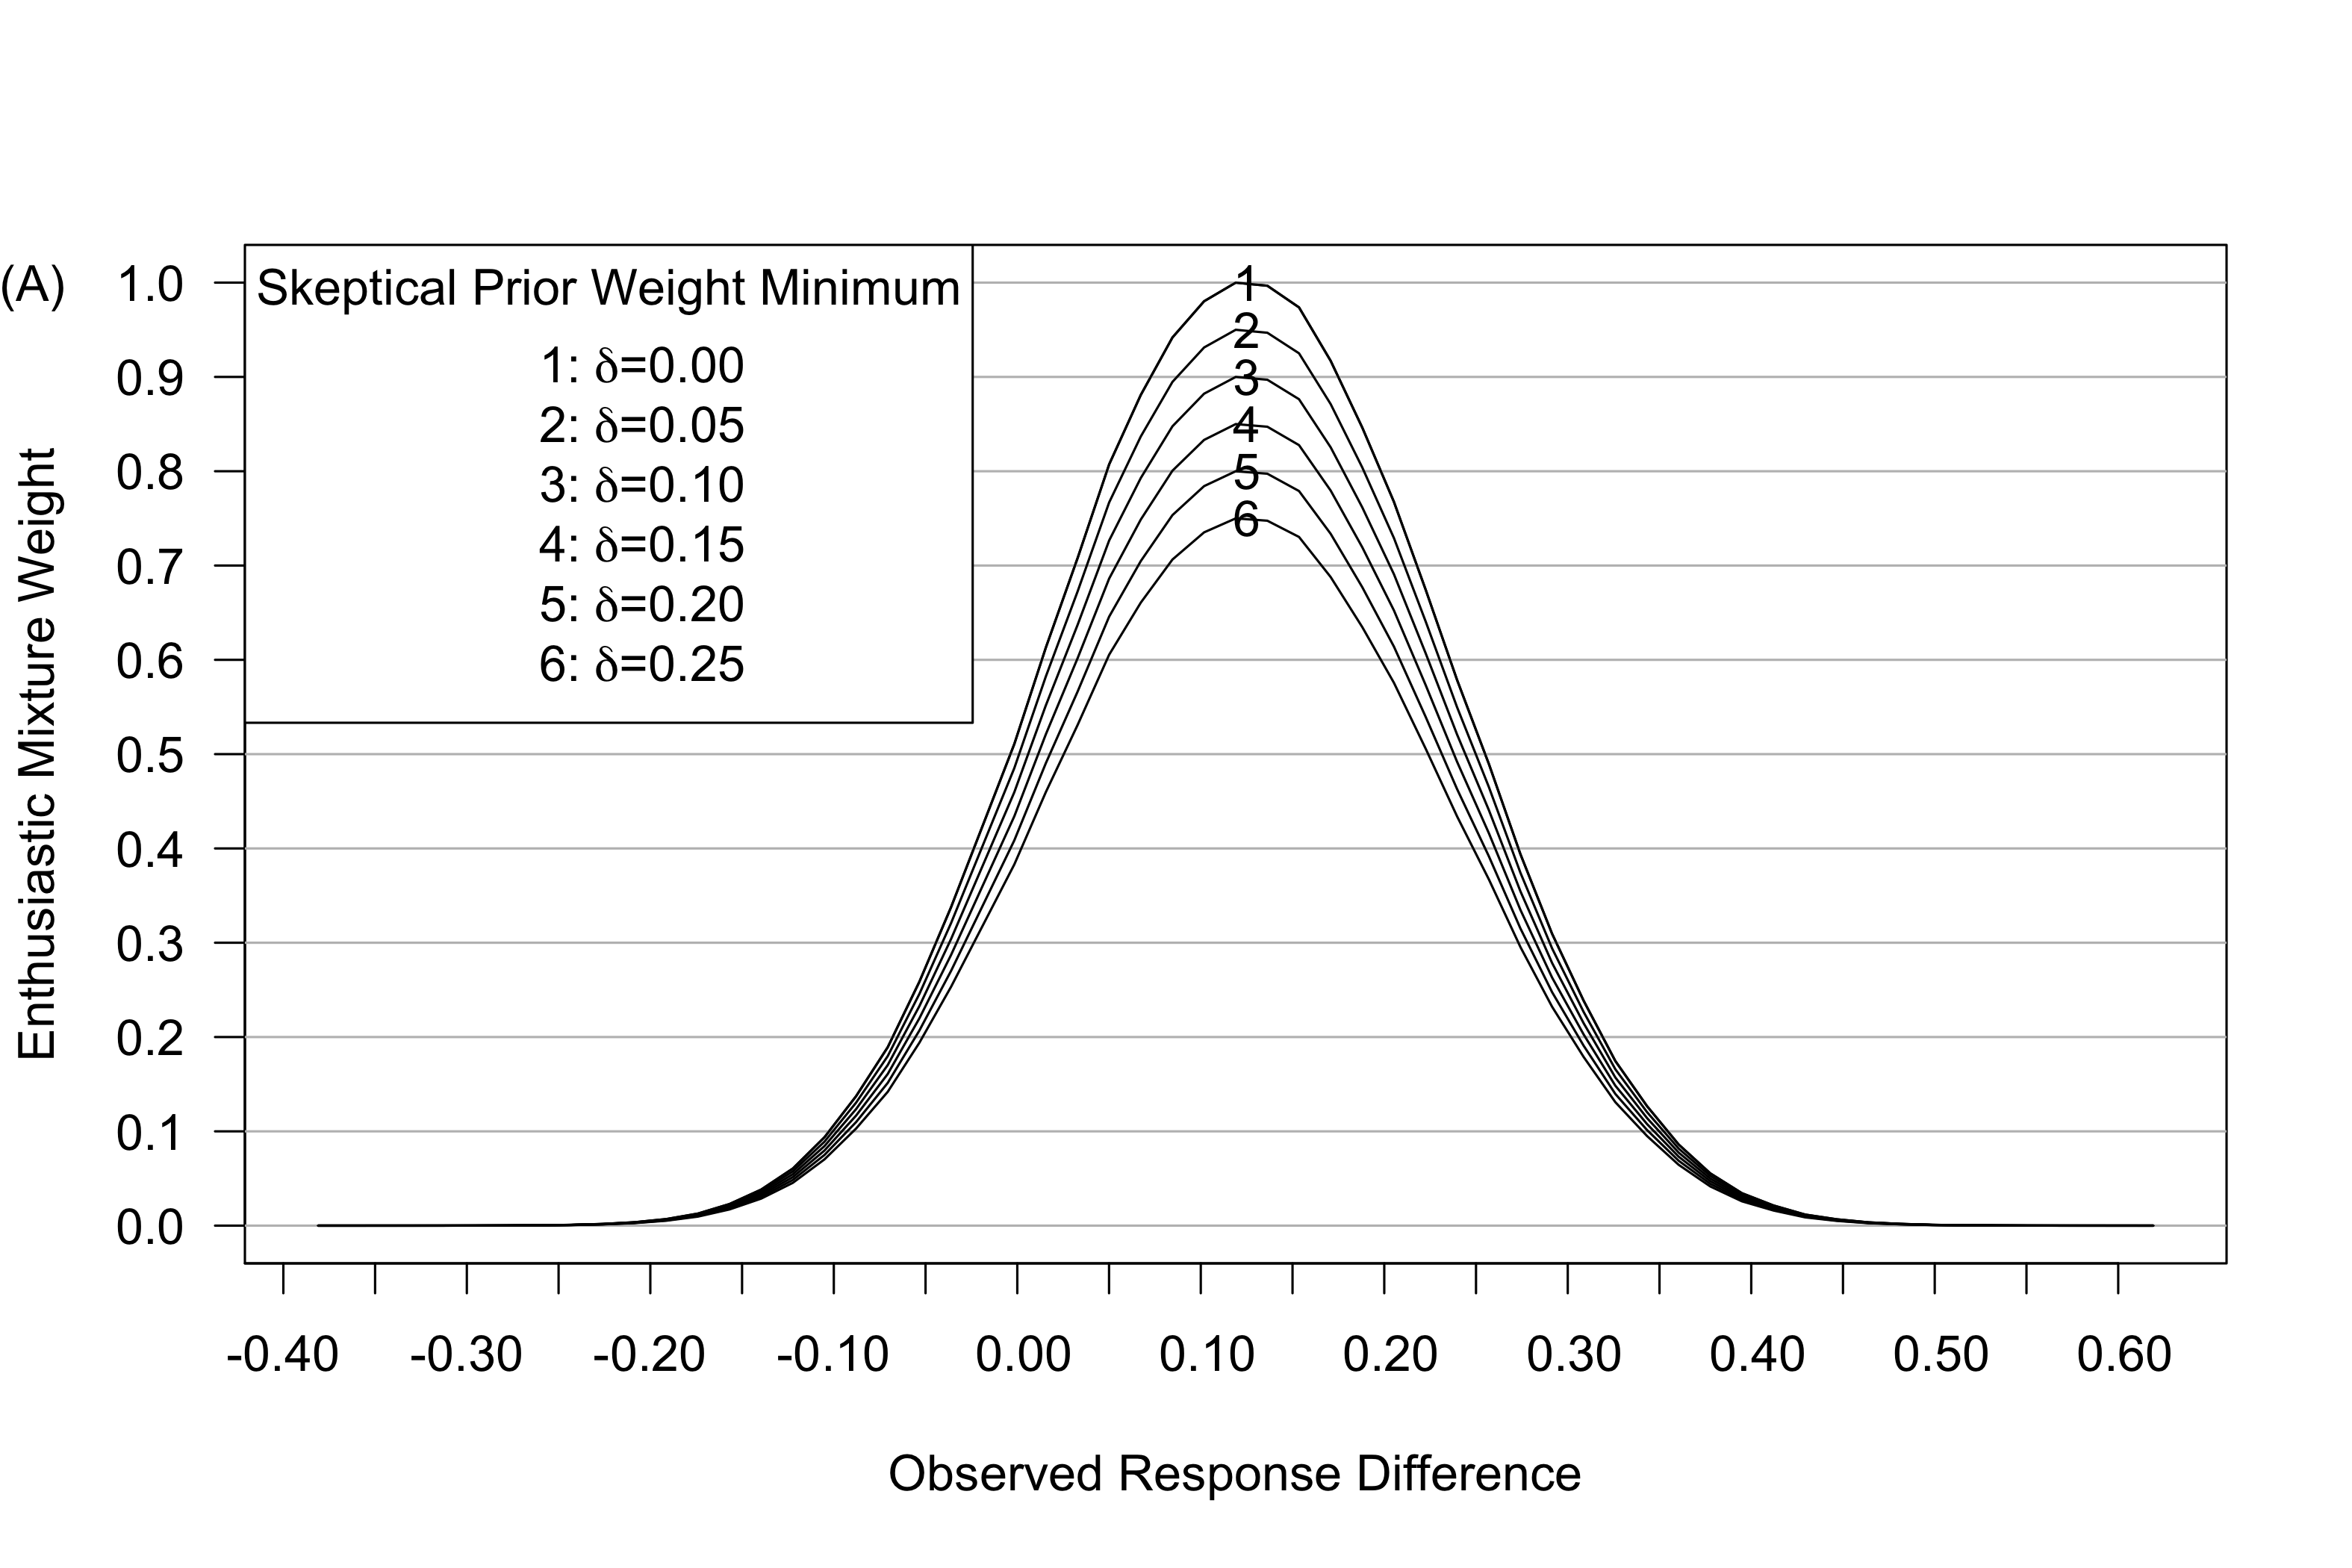
\includegraphics[width=0.75\textwidth]{./figures/3-part-compatibility-2.png}
%    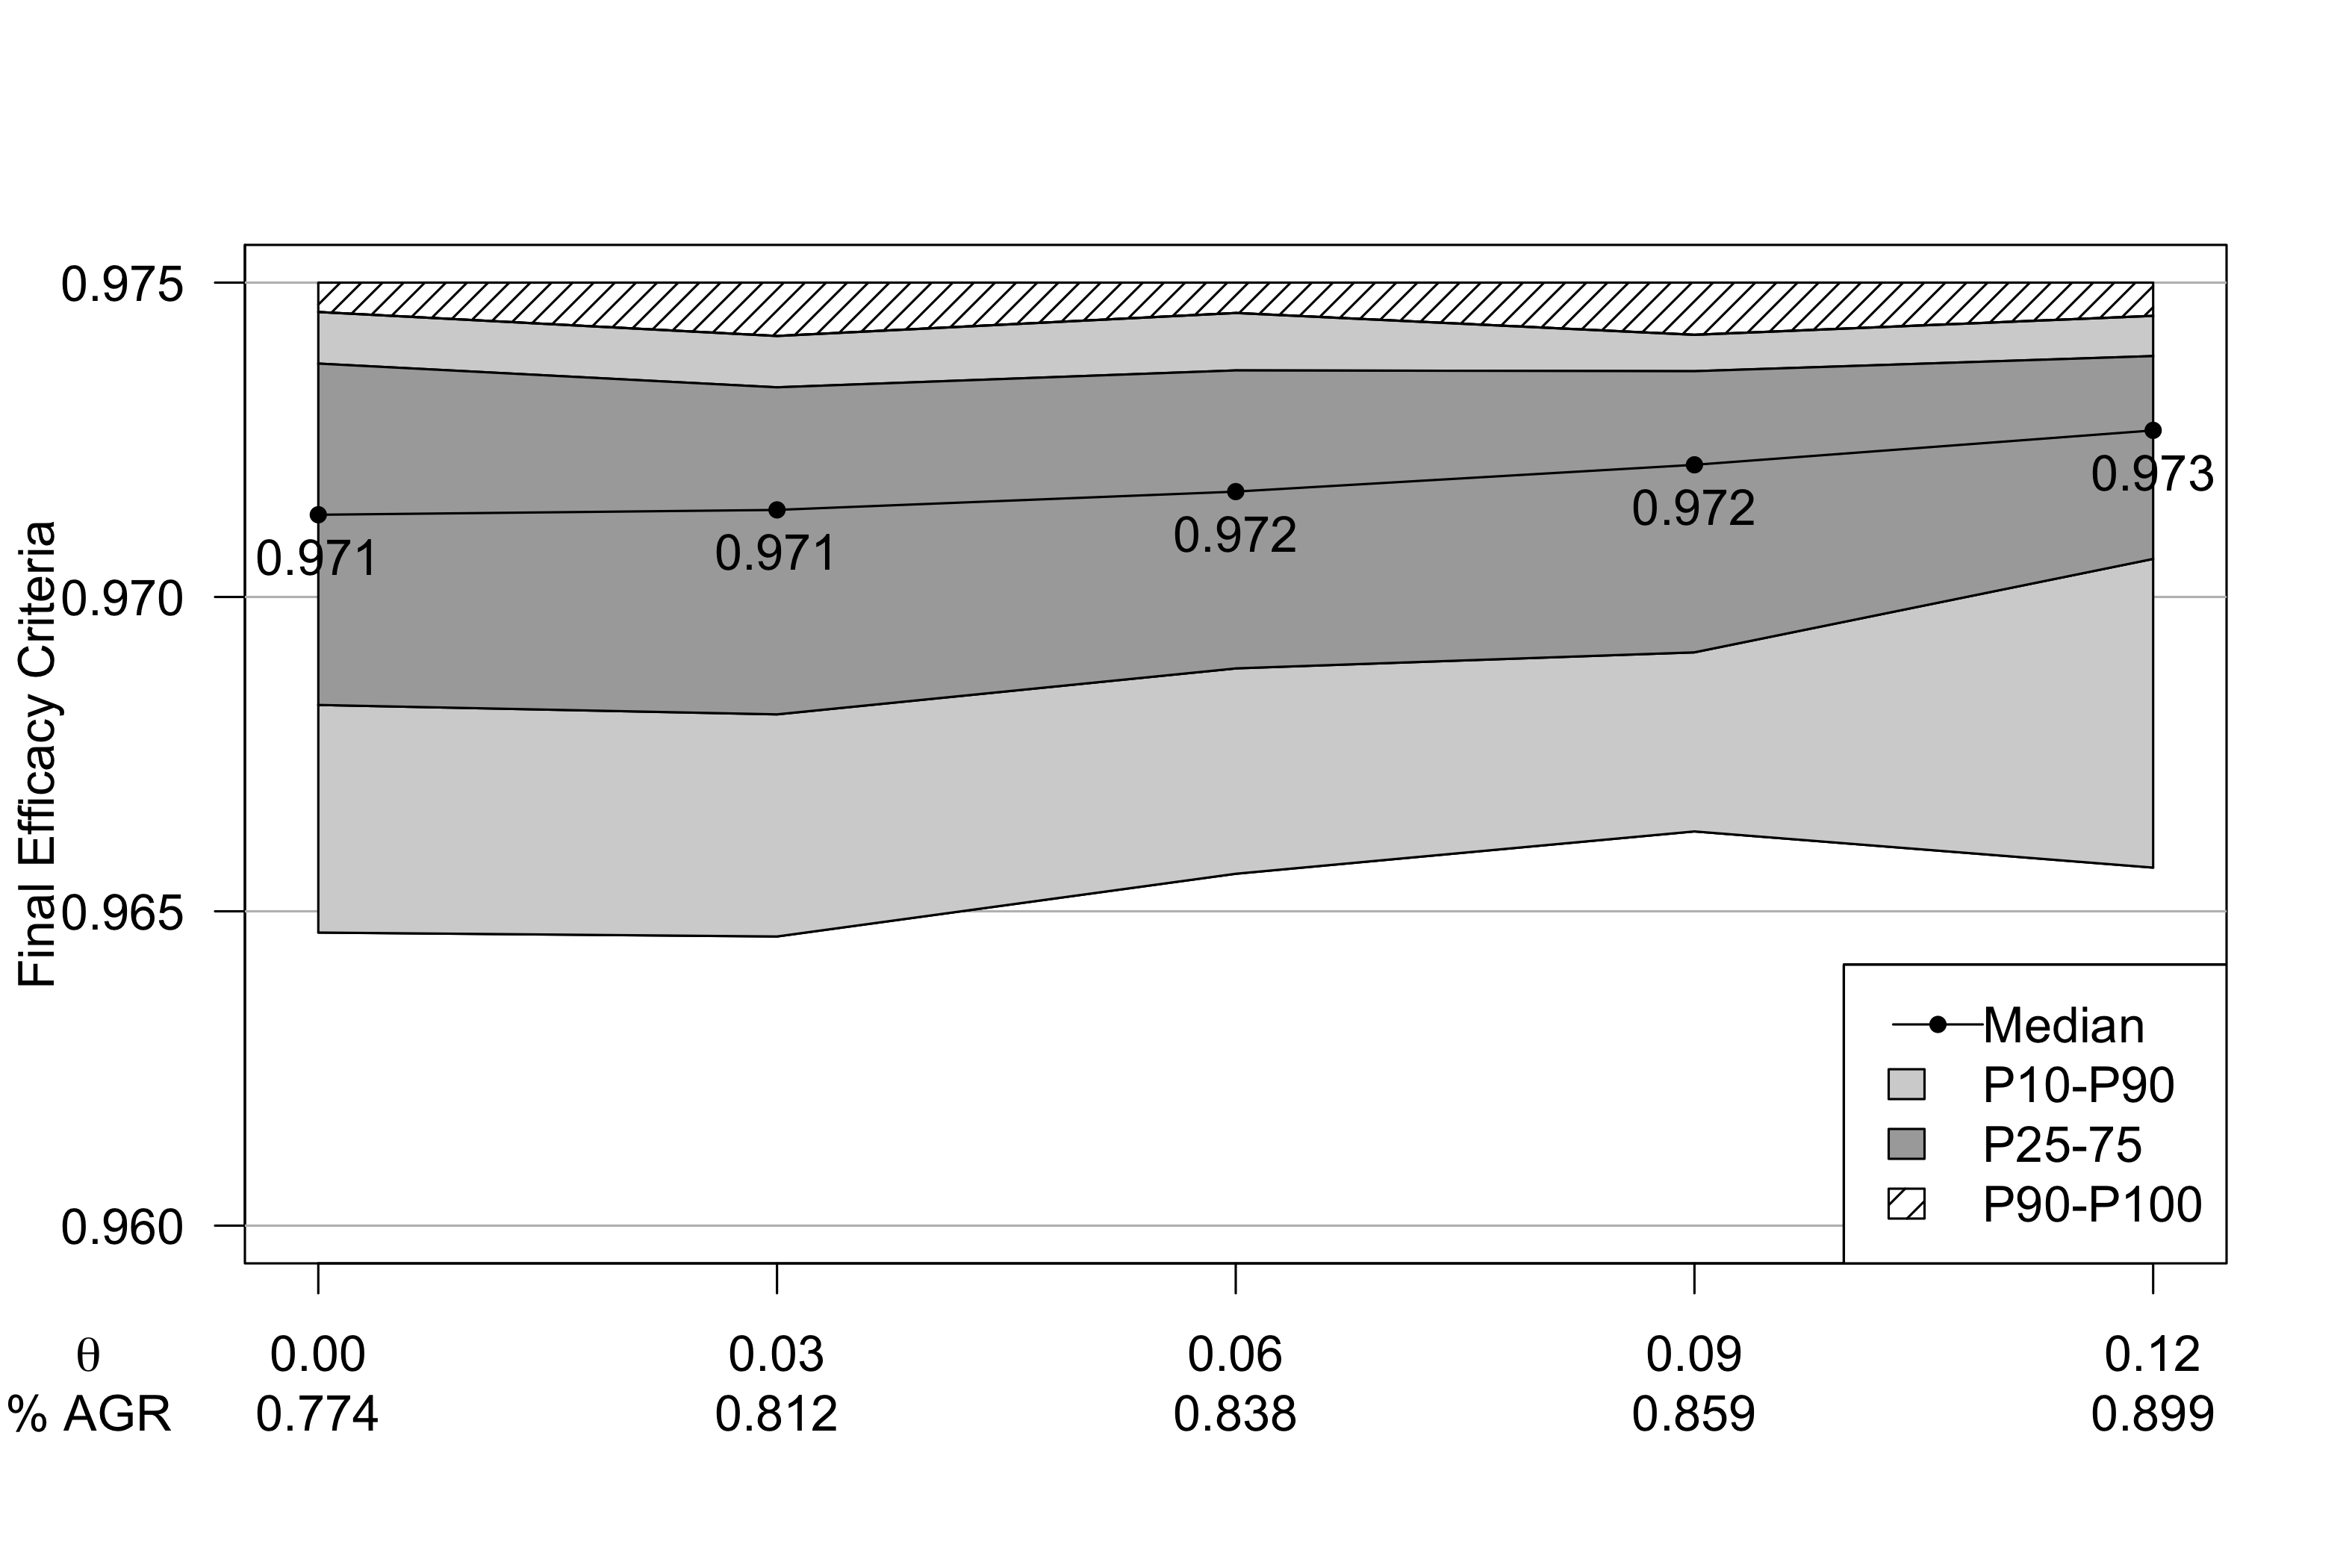
\includegraphics[width=6in]{figure6a.png}
    \caption{A, Enthusiastic prior mixing weight $\omega$ associated with skeptical prior weight minimum $\delta$ by observed response rate difference, when the placebo response rate is fixed at $38\%$.}
\label{fig:ex2varyomega}
 \end{center}
\end{figure}
\end{frame}

%\begin{frame}{Operating Characteristics}
%\begin{figure}[htbp]
%\begin{center}
%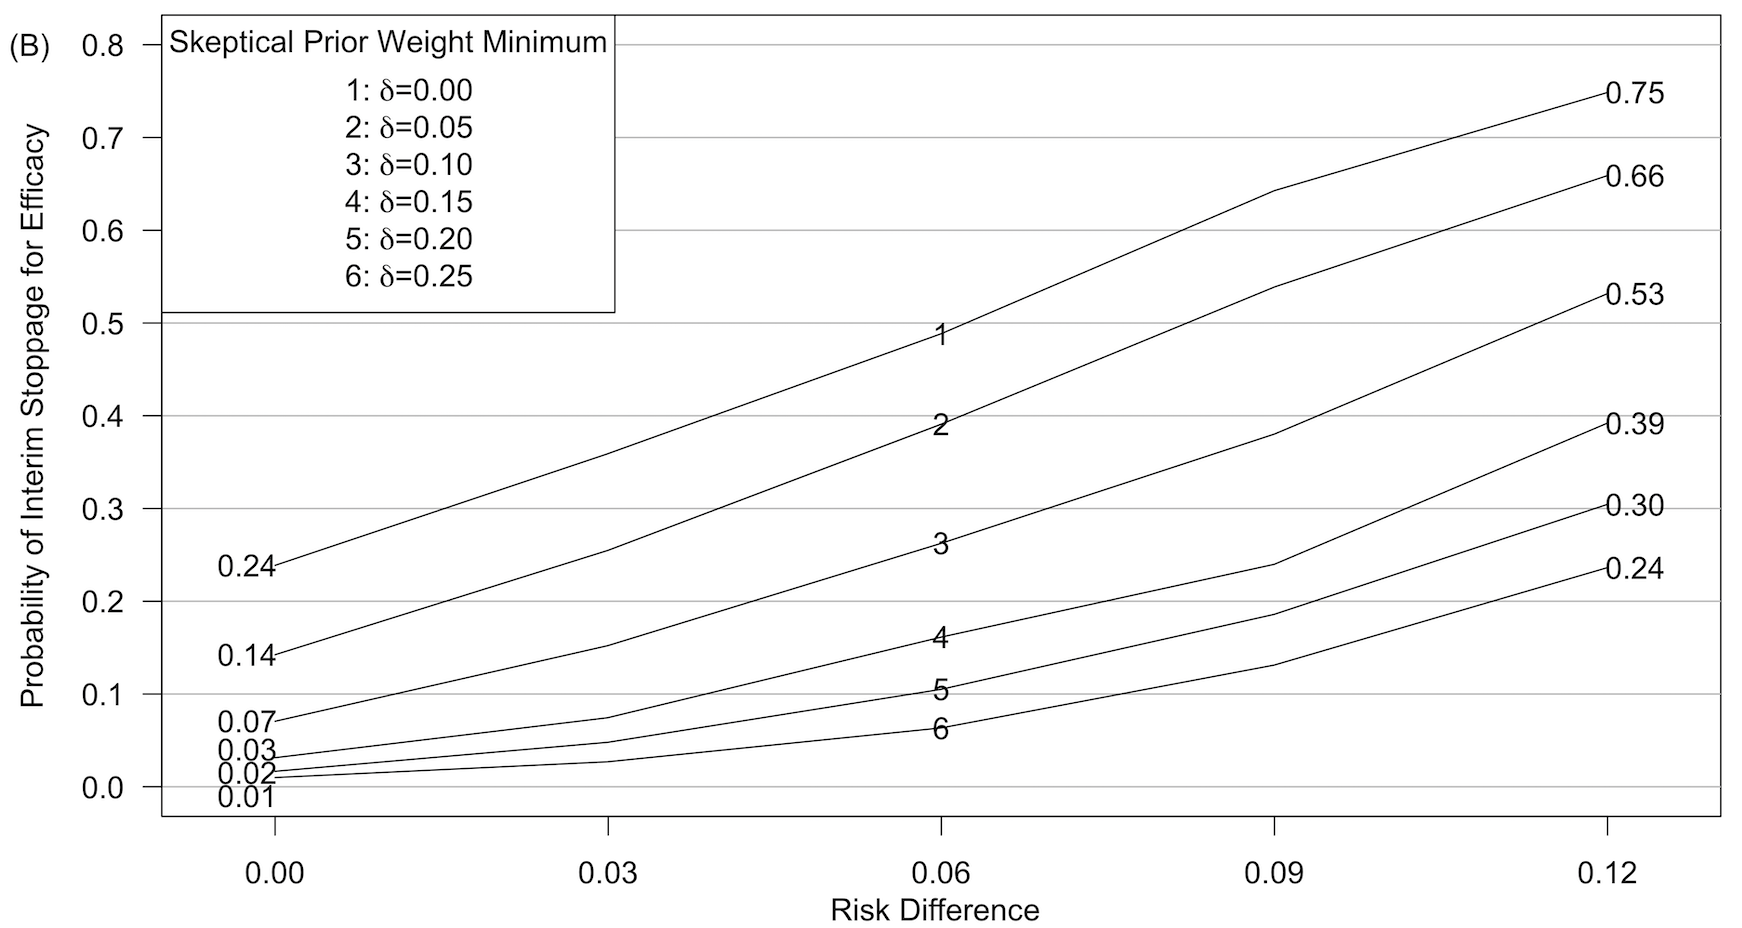
\includegraphics[width=1\textwidth]{./figures/aug12.png}
%%    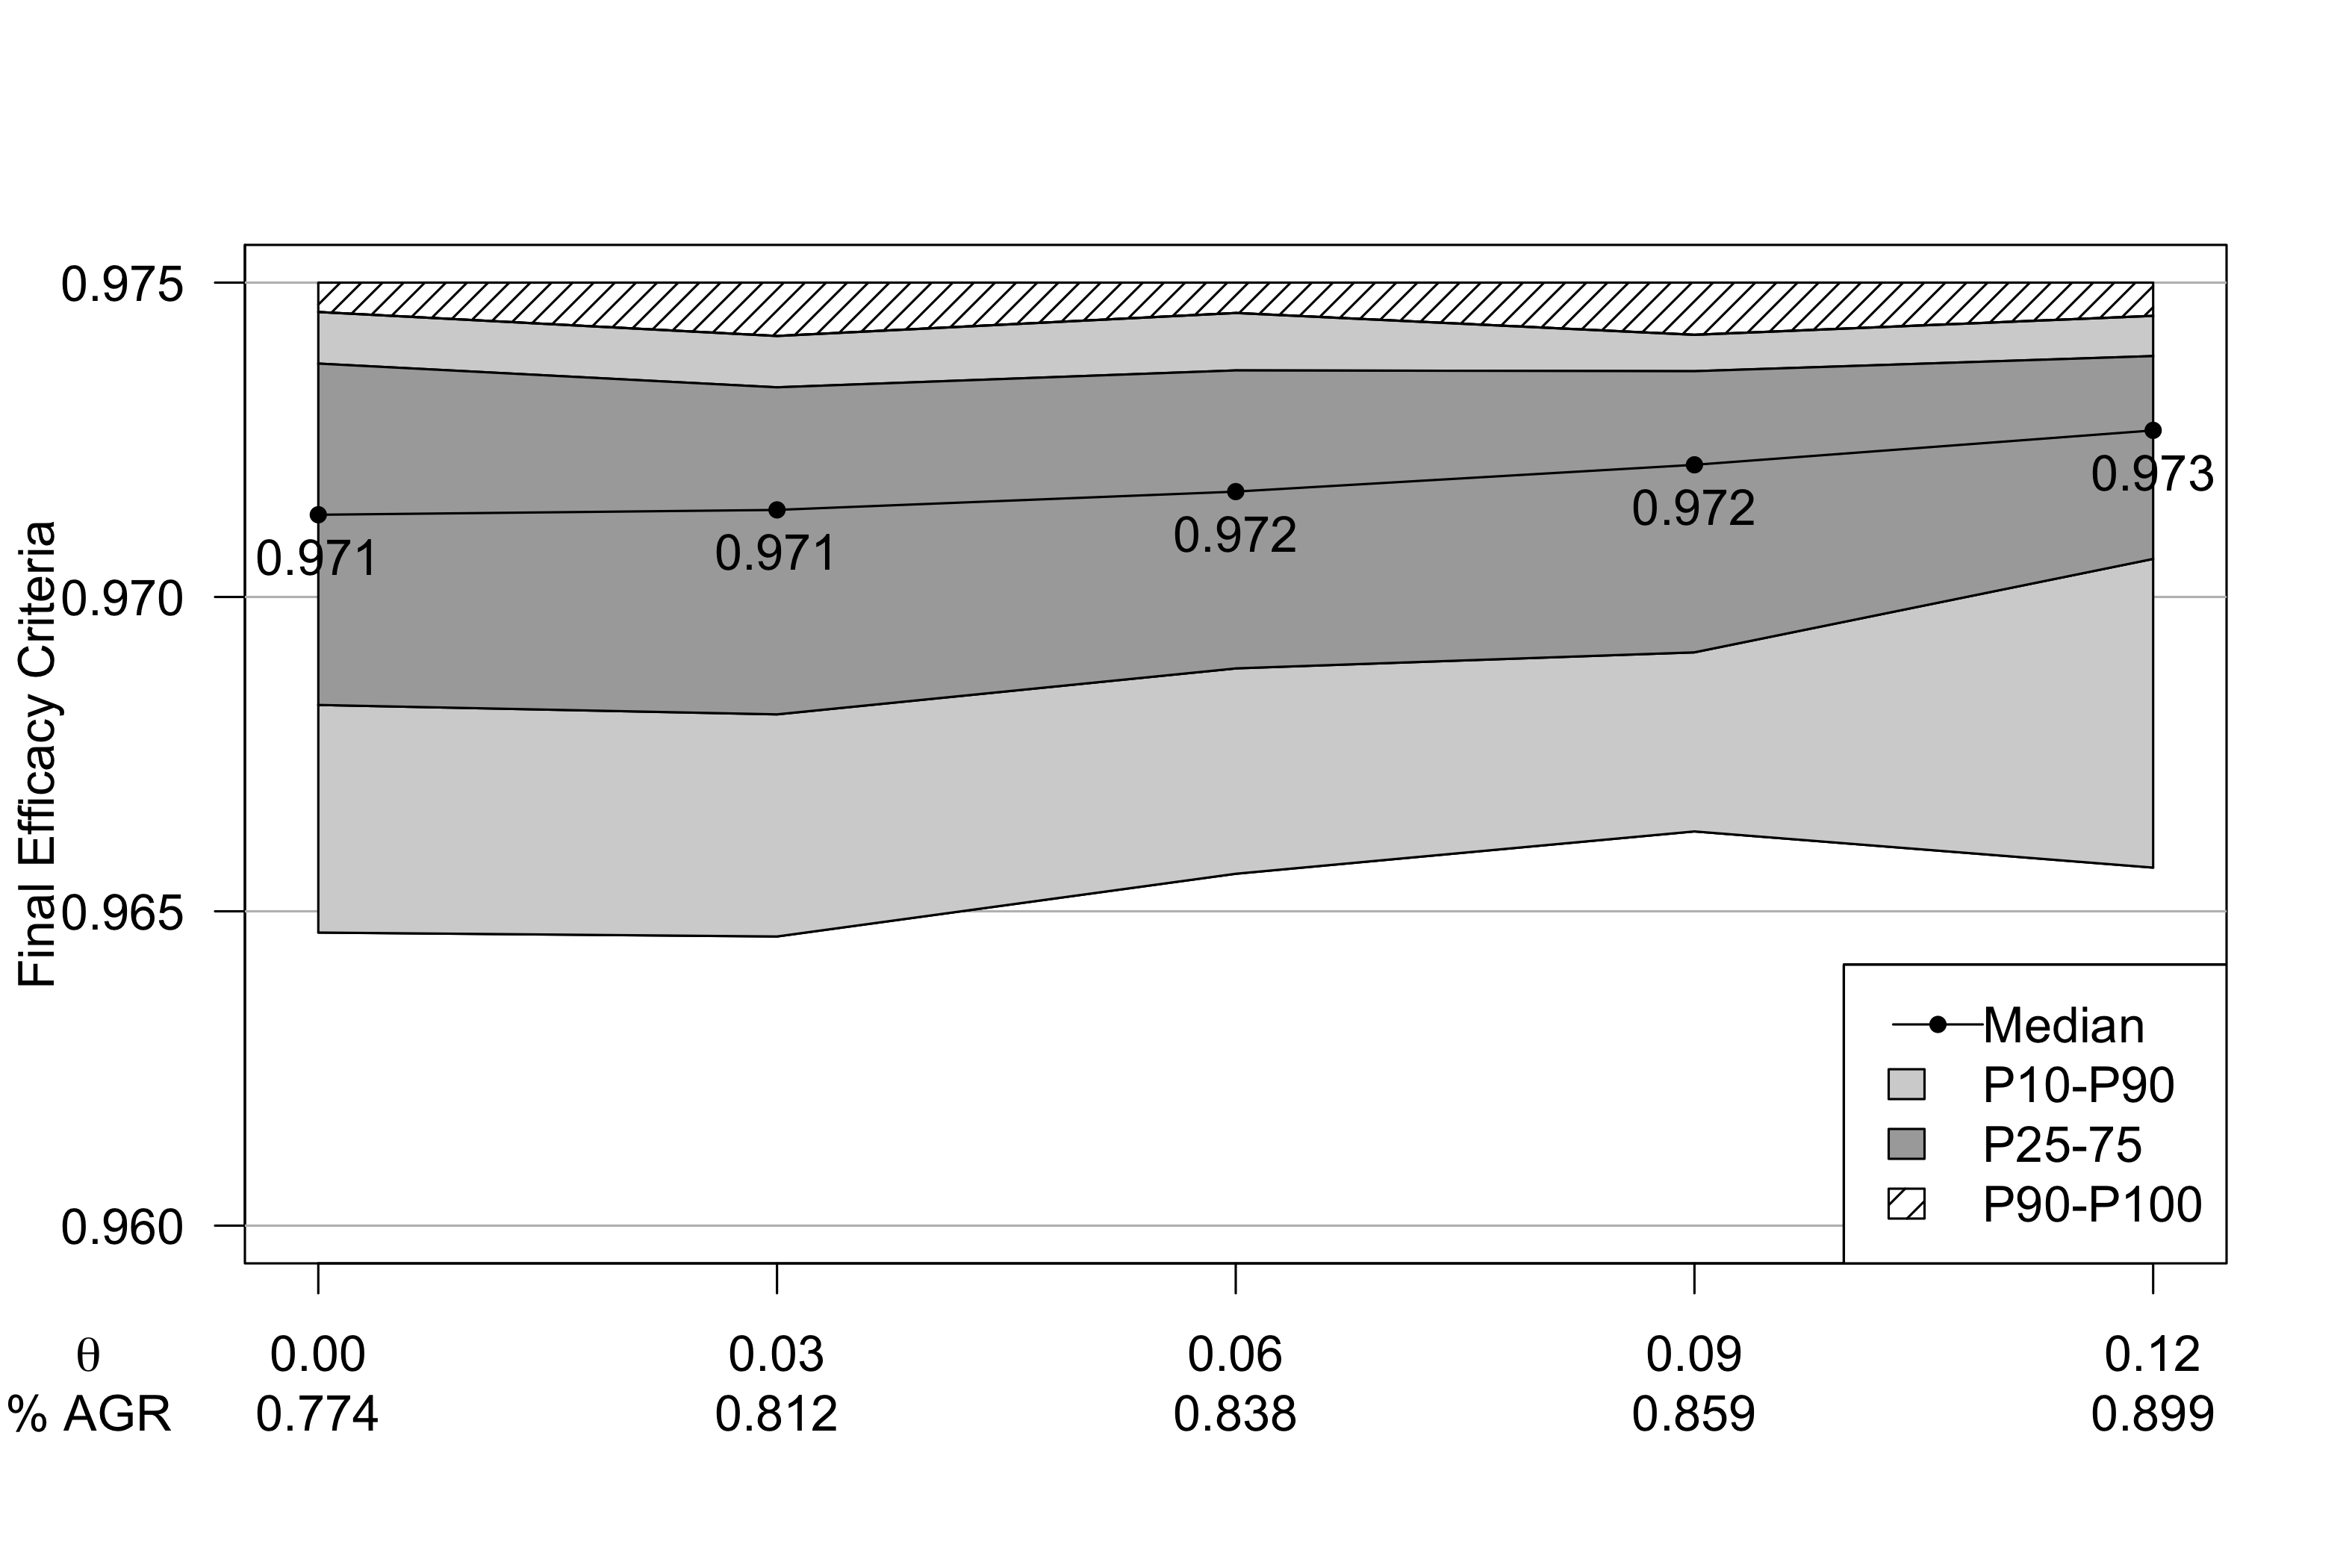
\includegraphics[width=6in]{figure6a.png}
%    \caption{B, Operating characteristics for designs having with skeptical prior weight minimum $\delta$ in \eqref{eq:omega} by true risk difference when the PC response rate generated at $39\%$.}
%\label{fig:ex2varyomega}
% \end{center}
%\end{figure}
%\end{frame}

\begin{frame}{Final PLUTO Trial Data}
\begin{itemize}
\item Ultimately, 93 patients were enrolled over approximately 52.5 months (approximately 1 patient enrolled per 17 days).
%
\vspace{0.5cm}
\item Clinical response was observed in 28 of 53 (52.8\%) of patients randomized to belimumab and in 17 of 40 (43.6\%) of patients randomized to placebo.

\vspace{0.5cm}
\item Posterior characteristics for response rate difference (using non-informative priors)
\begin{itemize}
  \vspace{0.5cm}
	\item Posterior Mean $\rightarrow$ 0.09
	
	\vspace{0.5cm}
	\item 95\% Credible Interval $\rightarrow$ [-0.11, 0.30]
\end{itemize}
\end{itemize}
\end{frame}

\begin{frame}{Re-analysis of Accumulating PLUTO Trial Data}
\footnotesize
\begin{table}[htbp]\label{tbl:real-pluto}%
\centering
\caption{Summary characteristics of re-analysis of PLUTO trial.}%
\begin{tabular*}{300pt}{@{\extracolsep\fill}cccccc@{\extracolsep\fill}}%
\toprule
$\delta$	&	SS (I/F)			&	$\psi^{(E)}(\mathbf{D}_{\text{obs}})$ (I/F)			&	$\omega$ (I/F)			&	$P(\theta>\theta_0=0)$ (I/F)			\\
\midrule
0.00	&	62	/	90	&	0.914	/	0.965	&	0.914	/	0.965	&	0.980	/	0.979	\\
0.05	&	64	/	92	&	0.876	/	0.934	&	0.833	/	0.887	&	0.976	/	0.962	\\
0.10	&	76	/	92	&	0.941	/	0.934	&	0.847	/	0.841	&	0.975	/	0.951	\\
0.15	&	92	/	92	&	0.934	/	0.934	&	0.794	/	0.794	&	0.940	/	0.940	\\
0.20	&	92	/	92	&	0.934	/	0.934	&	0.747	/	0.747	&	0.928	/	0.928	\\
0.25	&	92	/	92	&	0.934	/	0.934	&	0.701	/	0.701	&	0.917	/	0.917	\\
\bottomrule
\end{tabular*}
\end{table}
\hspace{0.75cm} SS = Sample Size, I/F = Interim/Final.
\end{frame}

\begin{frame}{Box's $P$-value Using Enthusiastic Prior $\psi^{(E)}(\mathbf{D}_{\text{obs}})$ }

\vspace{-0.3cm}
\begin{figure}[htbp]
\begin{center}
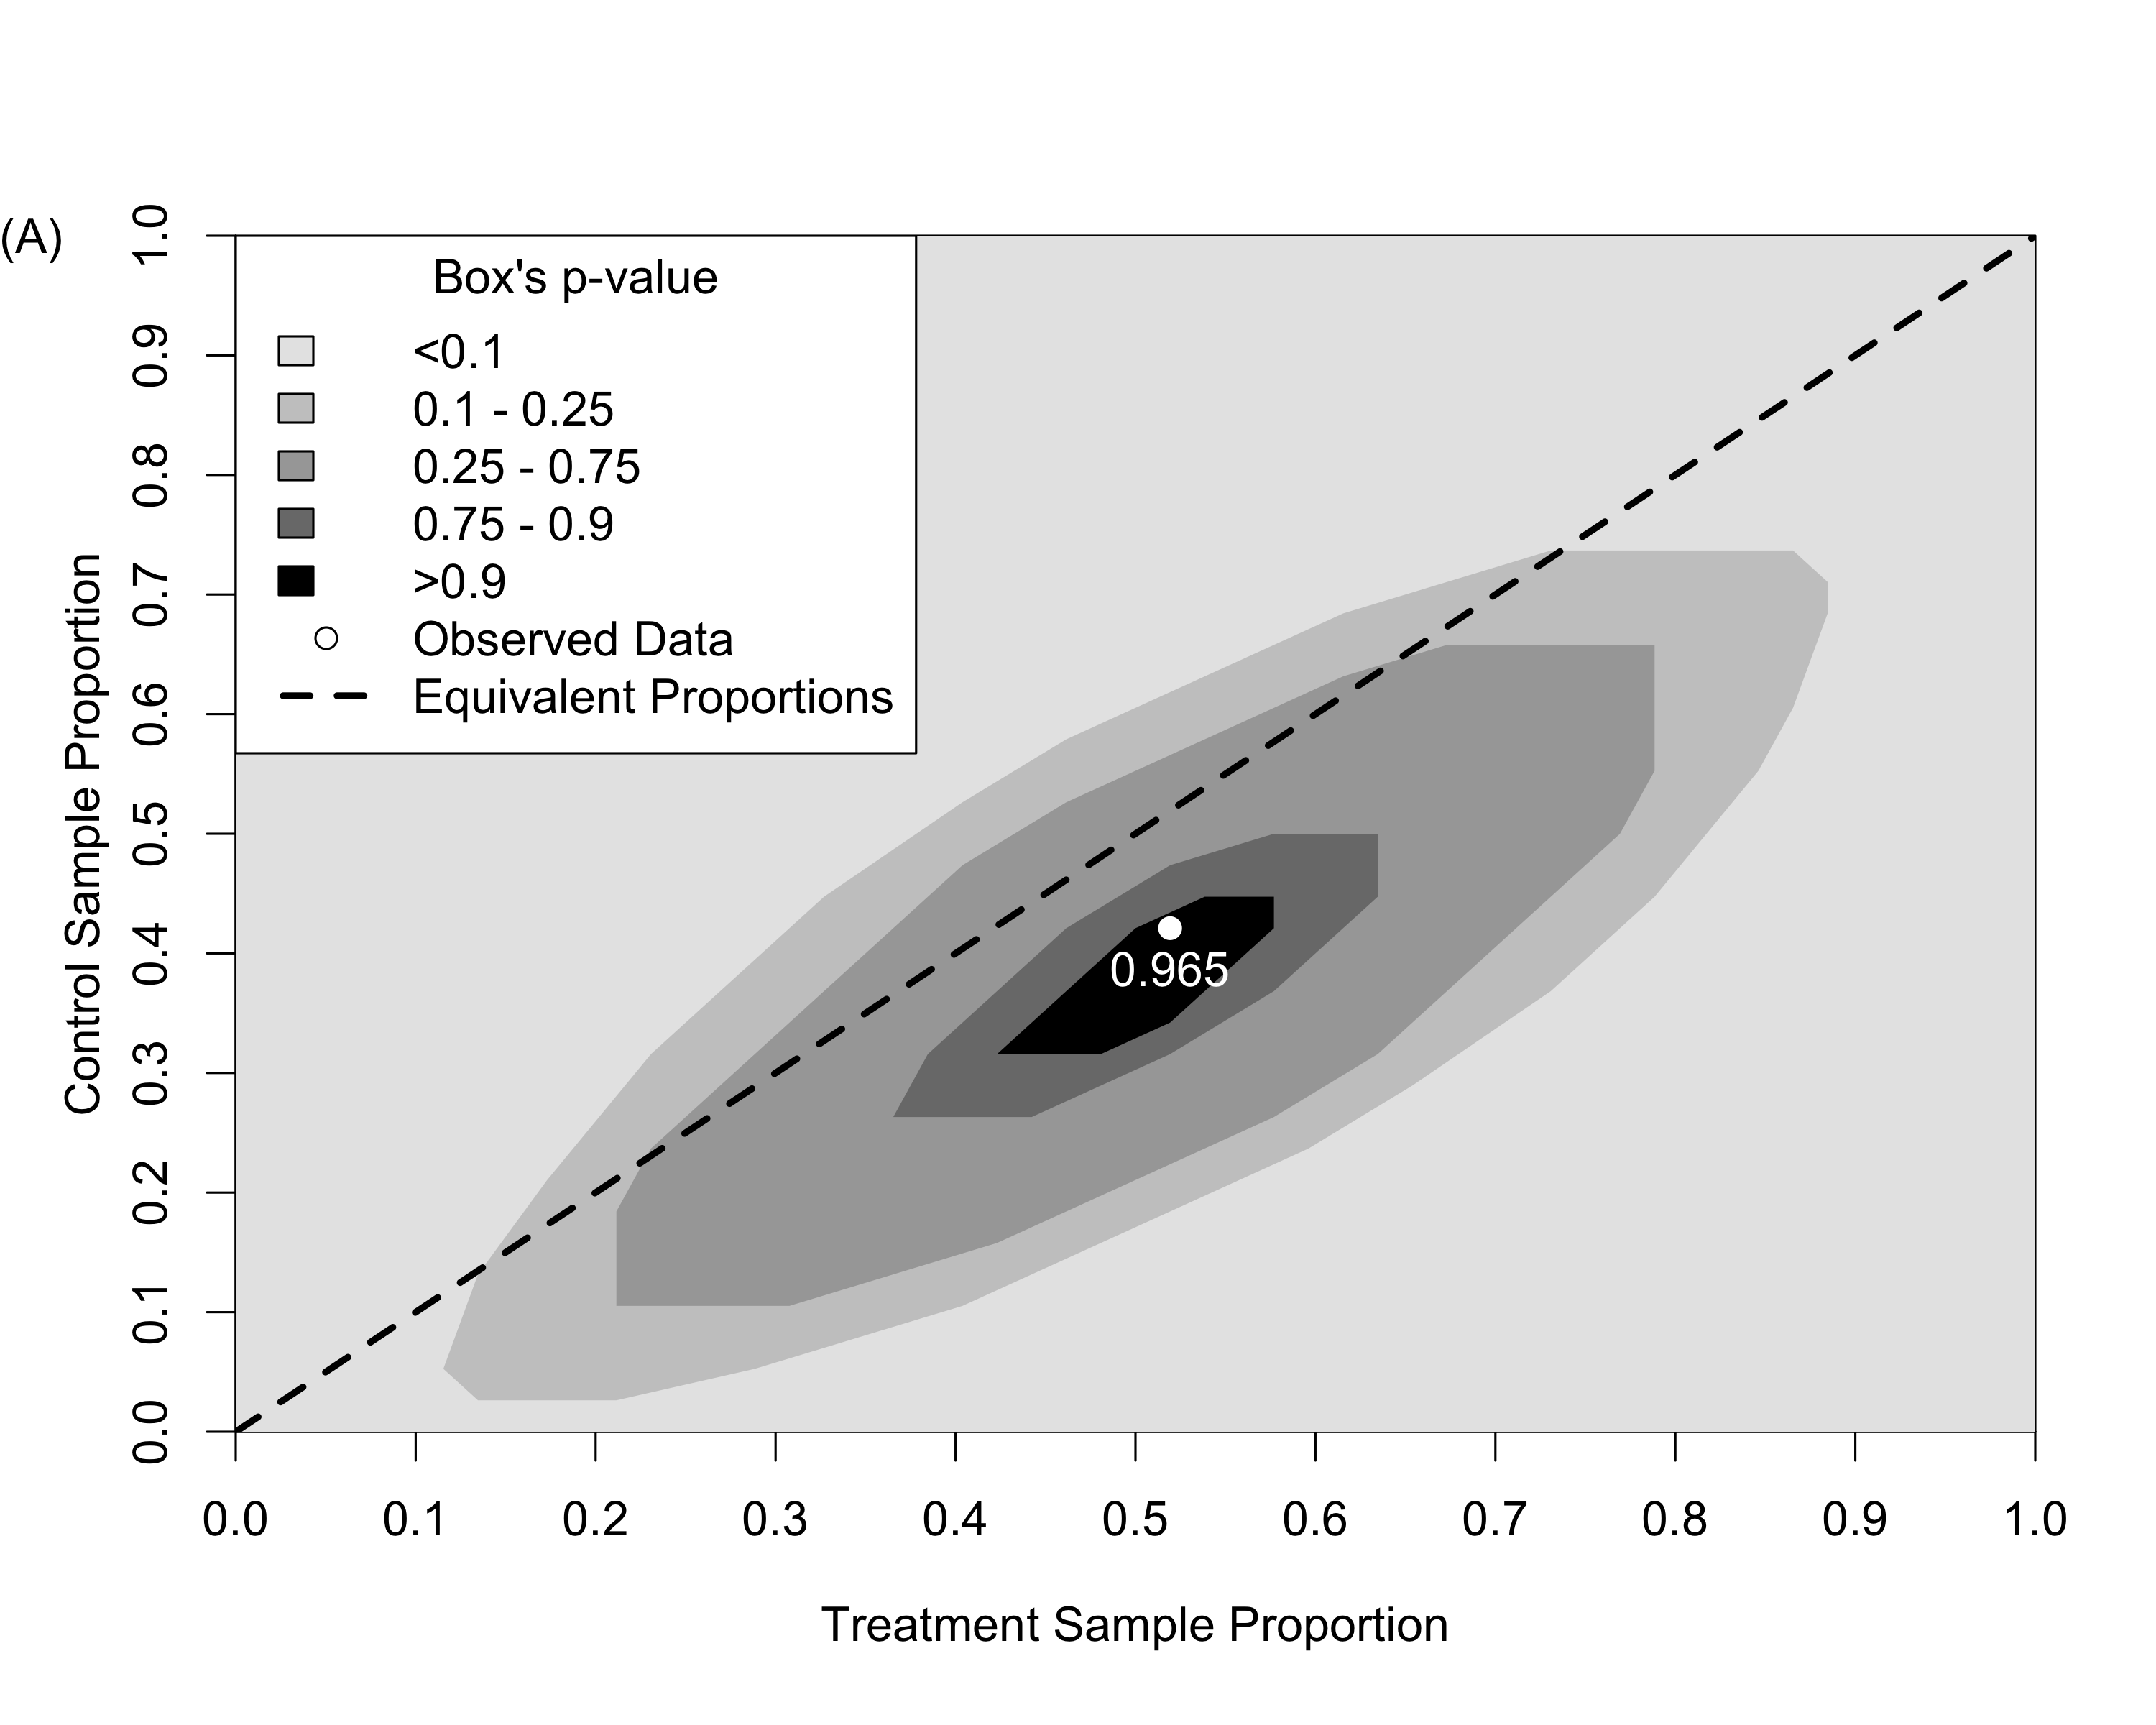
\includegraphics[width=0.7\textwidth]{./figures/2dbayesp.png}
    \caption{A, Values of $\psi^{(E)}(\mathbf{D}_{\text{obs}})$ by control and treatment sample proportions at the final analysis with 90 subjects for the $\delta=0$ case.}
\label{fig:2dheatmaps}
 \end{center}
\end{figure}
\end{frame}

\begin{frame}{Posterior Probability of Treatment Efficacy}

\vspace{-0.3cm}
\begin{figure}[htbp]
\begin{center}
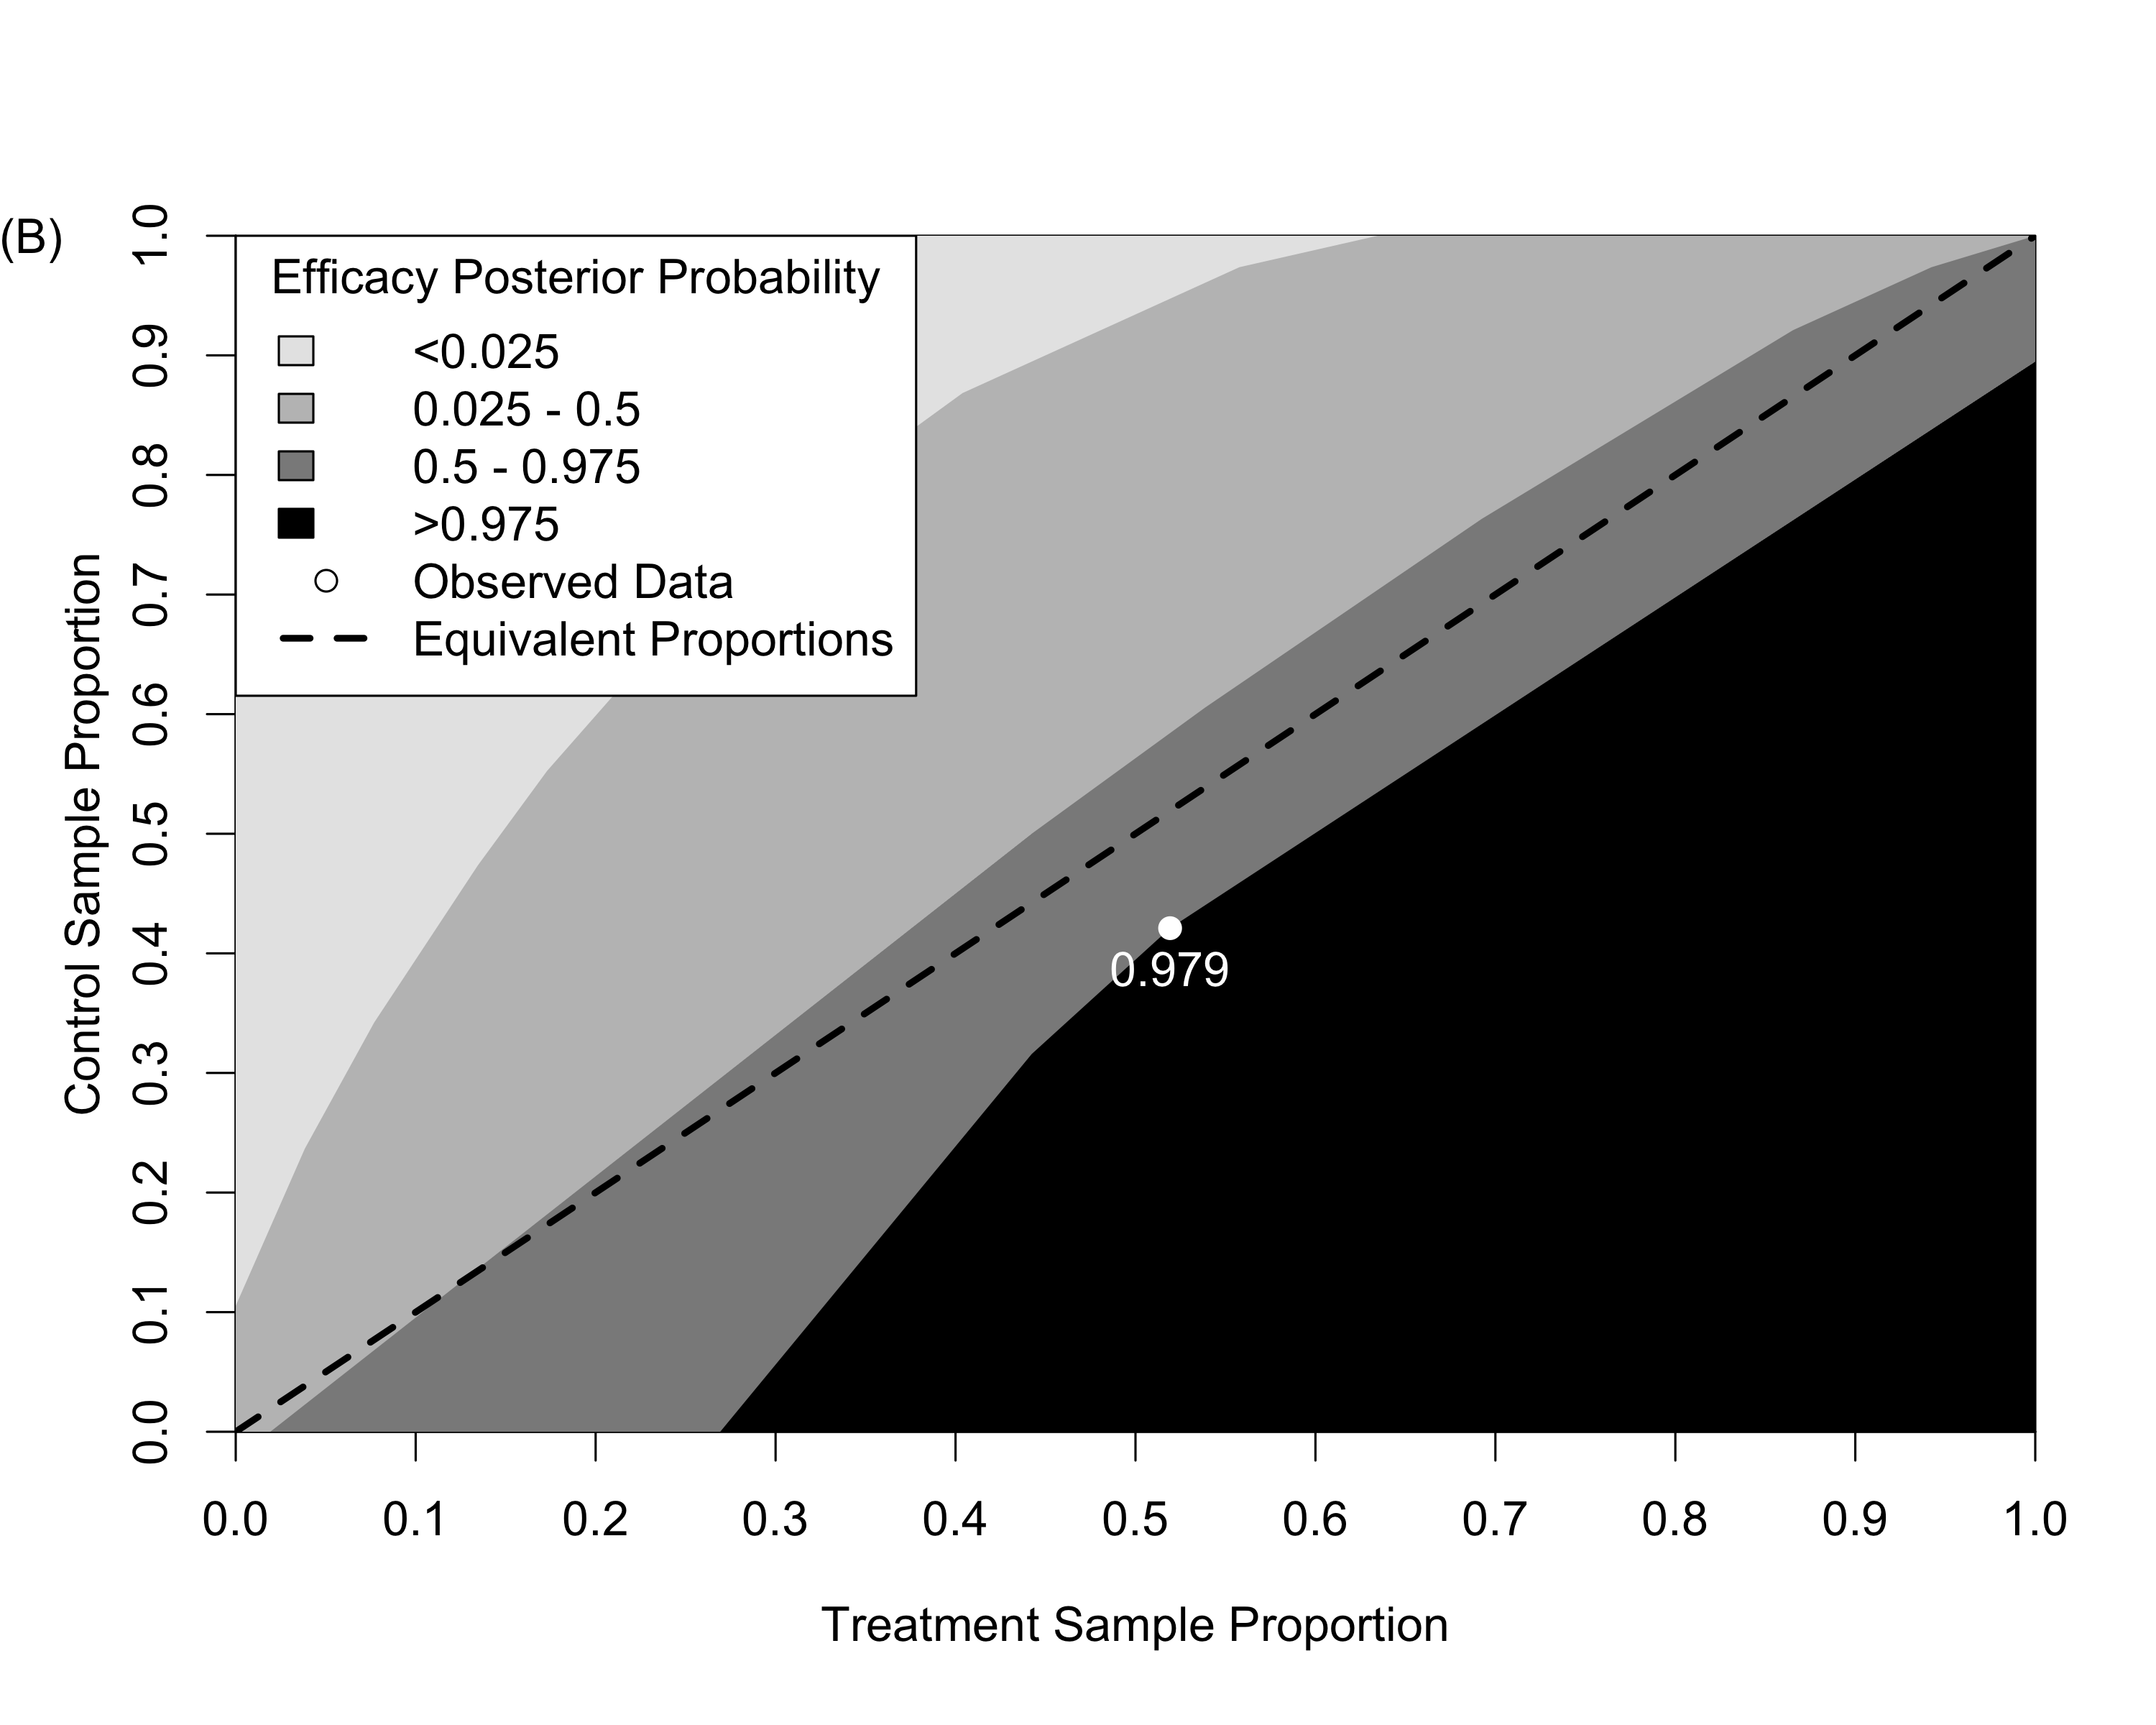
\includegraphics[width=0.7\textwidth]{./figures/2dpostp.png}
    \caption{B, $P(\theta>\theta_0=0)$ by control and treatment sample proportions at the final analysis with 90 subjects for the $\delta=0$ case.}
\label{fig:2dheatmaps}
 \end{center}
\end{figure}
\end{frame}


\section{Closing Remarks}

\begin{frame} \frametitle{Closing Remarks}
		\begin{itemize}
			\item The formulation of the enthusiastic prior enforces that there be residual uncertainty 
						that the null hypothesis is true; it demonstrates strong belief about effectiveness 
						of the treatment yet is still consistent with a modicum of equipoise.
			
			\vspace{0.75cm}	
			\item Even in the most liberal case where $\delta=0$, the residual uncertainty that the null hypothesis is true 
						reflected in the adaptive monitoring prior cannot be less than that reflected in the 
						enthusiastic prior.
			
			\vspace{0.75cm}	
			\item This is a critical feature of the design as it enforces the requirement that observed data 
			      must demonstrate some degree of efficacy on their own to justify stopping enrollment early.
		 \end{itemize}
\end{frame}


\begin{frame}[t,allowframebreaks]{References}
%\bibliographystyle{agsm} 
\bibliographystyle{natbib}
\bibliography{./References}	
%\bibliography{FinalDissertationReferences.bib}
\end{frame}

\end{document}